\documentclass[twoside]{book}

% Packages required by doxygen
\usepackage{fixltx2e}
\usepackage{calc}
\usepackage{doxygen}
\usepackage[export]{adjustbox} % also loads graphicx
\usepackage{graphicx}
\usepackage[utf8]{inputenc}
\usepackage{makeidx}
\usepackage{multicol}
\usepackage{multirow}
\PassOptionsToPackage{warn}{textcomp}
\usepackage{textcomp}
\usepackage[nointegrals]{wasysym}
\usepackage[table]{xcolor}

% Font selection
\usepackage[T1]{fontenc}
\usepackage[scaled=.90]{helvet}
\usepackage{courier}
\usepackage{amssymb}
\usepackage{sectsty}
\renewcommand{\familydefault}{\sfdefault}
\allsectionsfont{%
  \fontseries{bc}\selectfont%
  \color{darkgray}%
}
\renewcommand{\DoxyLabelFont}{%
  \fontseries{bc}\selectfont%
  \color{darkgray}%
}
\newcommand{\+}{\discretionary{\mbox{\scriptsize$\hookleftarrow$}}{}{}}

% Page & text layout
\usepackage{geometry}
\geometry{%
  a4paper,%
  top=2.5cm,%
  bottom=2.5cm,%
  left=2.5cm,%
  right=2.5cm%
}
\tolerance=750
\hfuzz=15pt
\hbadness=750
\setlength{\emergencystretch}{15pt}
\setlength{\parindent}{0cm}
\setlength{\parskip}{3ex plus 2ex minus 2ex}
\makeatletter
\renewcommand{\paragraph}{%
  \@startsection{paragraph}{4}{0ex}{-1.0ex}{1.0ex}{%
    \normalfont\normalsize\bfseries\SS@parafont%
  }%
}
\renewcommand{\subparagraph}{%
  \@startsection{subparagraph}{5}{0ex}{-1.0ex}{1.0ex}{%
    \normalfont\normalsize\bfseries\SS@subparafont%
  }%
}
\makeatother

% Headers & footers
\usepackage{fancyhdr}
\pagestyle{fancyplain}
\fancyhead[LE]{\fancyplain{}{\bfseries\thepage}}
\fancyhead[CE]{\fancyplain{}{}}
\fancyhead[RE]{\fancyplain{}{\bfseries\leftmark}}
\fancyhead[LO]{\fancyplain{}{\bfseries\rightmark}}
\fancyhead[CO]{\fancyplain{}{}}
\fancyhead[RO]{\fancyplain{}{\bfseries\thepage}}
\fancyfoot[LE]{\fancyplain{}{}}
\fancyfoot[CE]{\fancyplain{}{}}
\fancyfoot[RE]{\fancyplain{}{\bfseries\scriptsize Generated by Doxygen }}
\fancyfoot[LO]{\fancyplain{}{\bfseries\scriptsize Generated by Doxygen }}
\fancyfoot[CO]{\fancyplain{}{}}
\fancyfoot[RO]{\fancyplain{}{}}
\renewcommand{\footrulewidth}{0.4pt}
\renewcommand{\chaptermark}[1]{%
  \markboth{#1}{}%
}
\renewcommand{\sectionmark}[1]{%
  \markright{\thesection\ #1}%
}

% Indices & bibliography
\usepackage{natbib}
\usepackage[titles]{tocloft}
\setcounter{tocdepth}{3}
\setcounter{secnumdepth}{5}
\makeindex

% Hyperlinks (required, but should be loaded last)
\usepackage{ifpdf}
\ifpdf
  \usepackage[pdftex,pagebackref=true]{hyperref}
\else
  \usepackage[ps2pdf,pagebackref=true]{hyperref}
\fi
\hypersetup{%
  colorlinks=true,%
  linkcolor=blue,%
  citecolor=blue,%
  unicode%
}

% Custom commands
\newcommand{\clearemptydoublepage}{%
  \newpage{\pagestyle{empty}\cleardoublepage}%
}

\usepackage{caption}
\captionsetup{labelsep=space,justification=centering,font={bf},singlelinecheck=off,skip=4pt,position=top}

%===== C O N T E N T S =====

\begin{document}

% Titlepage & ToC
\hypersetup{pageanchor=false,
             bookmarksnumbered=true,
             pdfencoding=unicode
            }
\pagenumbering{alph}
\begin{titlepage}
\vspace*{7cm}
\begin{center}%
{\Large Tracore }\\
\vspace*{1cm}
{\large Generated by Doxygen 1.8.12}\\
\end{center}
\end{titlepage}
\clearemptydoublepage
\pagenumbering{roman}
\tableofcontents
\clearemptydoublepage
\pagenumbering{arabic}
\hypersetup{pageanchor=true}

%--- Begin generated contents ---
\chapter{Hierarchical Index}
\section{Class Hierarchy}
This inheritance list is sorted roughly, but not completely, alphabetically\+:\begin{DoxyCompactList}
\item \contentsline{section}{algo\+:\+:Berclaz}{\pageref{classalgo_1_1Berclaz}}{}
\item \contentsline{section}{core\+:\+:Detection\+Sequence}{\pageref{classcore_1_1DetectionSequence}}{}
\item \contentsline{section}{util\+:\+:File\+IO}{\pageref{classutil_1_1FileIO}}{}
\item \contentsline{section}{util\+:\+:Filter2D}{\pageref{classutil_1_1Filter2D}}{}
\item \contentsline{section}{util\+:\+:Grid}{\pageref{classutil_1_1Grid}}{}
\item \contentsline{section}{algo\+:\+:K\+Shortest\+Paths}{\pageref{classalgo_1_1KShortestPaths}}{}
\item \contentsline{section}{util\+:\+:Logger}{\pageref{classutil_1_1Logger}}{}
\item \contentsline{section}{util\+:\+:My\+Math}{\pageref{classutil_1_1MyMath}}{}
\item \contentsline{section}{algo\+:\+:N\+Stage}{\pageref{classalgo_1_1NStage}}{}
\item \contentsline{section}{core\+:\+:Object\+Data}{\pageref{classcore_1_1ObjectData}}{}
\begin{DoxyCompactList}
\item \contentsline{section}{core\+:\+:Object\+Data2D}{\pageref{classcore_1_1ObjectData2D}}{}
\begin{DoxyCompactList}
\item \contentsline{section}{core\+:\+:Object\+Data\+Angular}{\pageref{classcore_1_1ObjectDataAngular}}{}
\item \contentsline{section}{core\+:\+:Object\+Data\+Box}{\pageref{classcore_1_1ObjectDataBox}}{}
\end{DoxyCompactList}
\item \contentsline{section}{core\+:\+:Tracklet}{\pageref{classcore_1_1Tracklet}}{}
\end{DoxyCompactList}
\item \contentsline{section}{util\+:\+:Parser}{\pageref{classutil_1_1Parser}}{}
\item \contentsline{section}{util\+:\+:Visualizer}{\pageref{classutil_1_1Visualizer}}{}
\end{DoxyCompactList}

\chapter{Class Index}
\section{Class List}
Here are the classes, structs, unions and interfaces with brief descriptions\+:\begin{DoxyCompactList}
\item\contentsline{section}{\hyperlink{classcore_1_1DetectionSequence}{core\+::\+Detection\+Sequence} }{\pageref{classcore_1_1DetectionSequence}}{}
\item\contentsline{section}{\hyperlink{classutil_1_1FileIO}{util\+::\+File\+IO} }{\pageref{classutil_1_1FileIO}}{}
\item\contentsline{section}{\hyperlink{classutil_1_1Logger}{util\+::\+Logger} }{\pageref{classutil_1_1Logger}}{}
\item\contentsline{section}{\hyperlink{classutil_1_1MyMath}{util\+::\+My\+Math} }{\pageref{classutil_1_1MyMath}}{}
\item\contentsline{section}{\hyperlink{classcore_1_1ObjectData}{core\+::\+Object\+Data} }{\pageref{classcore_1_1ObjectData}}{}
\item\contentsline{section}{\hyperlink{classcore_1_1ObjectData3D}{core\+::\+Object\+Data3D} }{\pageref{classcore_1_1ObjectData3D}}{}
\item\contentsline{section}{\hyperlink{classcore_1_1ObjectDataAngular}{core\+::\+Object\+Data\+Angular} }{\pageref{classcore_1_1ObjectDataAngular}}{}
\item\contentsline{section}{\hyperlink{classcore_1_1ObjectDataMap}{core\+::\+Object\+Data\+Map} }{\pageref{classcore_1_1ObjectDataMap}}{}
\item\contentsline{section}{\hyperlink{classutil_1_1Parser}{util\+::\+Parser} }{\pageref{classutil_1_1Parser}}{}
\item\contentsline{section}{\hyperlink{classcore_1_1Tracklet}{core\+::\+Tracklet} }{\pageref{classcore_1_1Tracklet}}{}
\item\contentsline{section}{\hyperlink{classalgo_1_1TwoStage}{algo\+::\+Two\+Stage} }{\pageref{classalgo_1_1TwoStage}}{}
\end{DoxyCompactList}

\chapter{Class Documentation}
\hypertarget{classcore_1_1DetectionSequence}{}\section{core\+:\+:Detection\+Sequence Class Reference}
\label{classcore_1_1DetectionSequence}\index{core\+::\+Detection\+Sequence@{core\+::\+Detection\+Sequence}}


{\ttfamily \#include $<$Detection\+Sequence.\+h$>$}

\subsection*{Public Member Functions}
\begin{DoxyCompactItemize}
\item 
\hyperlink{classcore_1_1DetectionSequence_a2cbdc8db34fe87932653826fc8a3c1f7}{Detection\+Sequence} (const std\+::string \&name=\char`\"{}Detection\+Sequence\char`\"{})
\item 
void \hyperlink{classcore_1_1DetectionSequence_a3cc0fdf3281f34985f4762086293db72}{Add\+Object} (Object\+Data\+Ptr object\+\_\+data)
\item 
void \hyperlink{classcore_1_1DetectionSequence_ab62569a3e51d58457057deba12ef6892}{Clear} ()
\item 
std\+::string \hyperlink{classcore_1_1DetectionSequence_a8a1af3dee89766d06f4a4f74044082ad}{Get\+Name} () const
\item 
Object\+Data\+Ptr \hyperlink{classcore_1_1DetectionSequence_aab2b72c6e0a9ee14dba99d07116c1d86}{Get\+Object} (size\+\_\+t frame\+\_\+index, size\+\_\+t object\+\_\+index) const
\item 
size\+\_\+t \hyperlink{classcore_1_1DetectionSequence_a2417e4f2652a39245d6f2faa0ce19571}{Get\+Frame\+Count} () const
\item 
size\+\_\+t \hyperlink{classcore_1_1DetectionSequence_a99a1b693215c386c4716df12f6040100}{Get\+Object\+Count} (size\+\_\+t frame\+\_\+index) const
\end{DoxyCompactItemize}
\subsection*{Friends}
\begin{DoxyCompactItemize}
\item 
std\+::ostream \& \hyperlink{classcore_1_1DetectionSequence_a557132cfbb170daf47f5a890a0c5bac0}{operator$<$$<$} (std\+::ostream \&os, const \hyperlink{classcore_1_1DetectionSequence}{Detection\+Sequence} \&obj)
\end{DoxyCompactItemize}


\subsection{Detailed Description}
Class for storing a full sequence of frame, each with multiple detected objects. 

\subsection{Constructor \& Destructor Documentation}
\index{core\+::\+Detection\+Sequence@{core\+::\+Detection\+Sequence}!Detection\+Sequence@{Detection\+Sequence}}
\index{Detection\+Sequence@{Detection\+Sequence}!core\+::\+Detection\+Sequence@{core\+::\+Detection\+Sequence}}
\subsubsection[{\texorpdfstring{Detection\+Sequence(const std\+::string \&name=""Detection\+Sequence"")}{DetectionSequence(const std::string \&name="DetectionSequence")}}]{\setlength{\rightskip}{0pt plus 5cm}core\+::\+Detection\+Sequence\+::\+Detection\+Sequence (
\begin{DoxyParamCaption}
\item[{const std\+::string \&}]{name = {\ttfamily \char`\"{}DetectionSequence\char`\"{}}}
\end{DoxyParamCaption}
)}\hypertarget{classcore_1_1DetectionSequence_a2cbdc8db34fe87932653826fc8a3c1f7}{}\label{classcore_1_1DetectionSequence_a2cbdc8db34fe87932653826fc8a3c1f7}
Creates a detection sequence with the given name. 
\begin{DoxyParams}{Parameters}
{\em name} & The name of this sequence \\
\hline
\end{DoxyParams}


\subsection{Member Function Documentation}
\index{core\+::\+Detection\+Sequence@{core\+::\+Detection\+Sequence}!Add\+Object@{Add\+Object}}
\index{Add\+Object@{Add\+Object}!core\+::\+Detection\+Sequence@{core\+::\+Detection\+Sequence}}
\subsubsection[{\texorpdfstring{Add\+Object(\+Object\+Data\+Ptr object\+\_\+data)}{AddObject(ObjectDataPtr object\_data)}}]{\setlength{\rightskip}{0pt plus 5cm}void core\+::\+Detection\+Sequence\+::\+Add\+Object (
\begin{DoxyParamCaption}
\item[{Object\+Data\+Ptr}]{object\+\_\+data}
\end{DoxyParamCaption}
)}\hypertarget{classcore_1_1DetectionSequence_a3cc0fdf3281f34985f4762086293db72}{}\label{classcore_1_1DetectionSequence_a3cc0fdf3281f34985f4762086293db72}
Adds a new object, creates a new frame vector if the given objects frame index is greater than the current frame vector size. 
\begin{DoxyParams}{Parameters}
{\em object\+\_\+data} & The object to add \\
\hline
\end{DoxyParams}
\index{core\+::\+Detection\+Sequence@{core\+::\+Detection\+Sequence}!Clear@{Clear}}
\index{Clear@{Clear}!core\+::\+Detection\+Sequence@{core\+::\+Detection\+Sequence}}
\subsubsection[{\texorpdfstring{Clear()}{Clear()}}]{\setlength{\rightskip}{0pt plus 5cm}void core\+::\+Detection\+Sequence\+::\+Clear (
\begin{DoxyParamCaption}
{}
\end{DoxyParamCaption}
)}\hypertarget{classcore_1_1DetectionSequence_ab62569a3e51d58457057deba12ef6892}{}\label{classcore_1_1DetectionSequence_ab62569a3e51d58457057deba12ef6892}
Removes all objects. \index{core\+::\+Detection\+Sequence@{core\+::\+Detection\+Sequence}!Get\+Frame\+Count@{Get\+Frame\+Count}}
\index{Get\+Frame\+Count@{Get\+Frame\+Count}!core\+::\+Detection\+Sequence@{core\+::\+Detection\+Sequence}}
\subsubsection[{\texorpdfstring{Get\+Frame\+Count() const}{GetFrameCount() const}}]{\setlength{\rightskip}{0pt plus 5cm}size\+\_\+t core\+::\+Detection\+Sequence\+::\+Get\+Frame\+Count (
\begin{DoxyParamCaption}
{}
\end{DoxyParamCaption}
) const}\hypertarget{classcore_1_1DetectionSequence_a2417e4f2652a39245d6f2faa0ce19571}{}\label{classcore_1_1DetectionSequence_a2417e4f2652a39245d6f2faa0ce19571}
Gets the frame count. \begin{DoxyReturn}{Returns}
The frame count 
\end{DoxyReturn}
\index{core\+::\+Detection\+Sequence@{core\+::\+Detection\+Sequence}!Get\+Name@{Get\+Name}}
\index{Get\+Name@{Get\+Name}!core\+::\+Detection\+Sequence@{core\+::\+Detection\+Sequence}}
\subsubsection[{\texorpdfstring{Get\+Name() const}{GetName() const}}]{\setlength{\rightskip}{0pt plus 5cm}std\+::string core\+::\+Detection\+Sequence\+::\+Get\+Name (
\begin{DoxyParamCaption}
{}
\end{DoxyParamCaption}
) const}\hypertarget{classcore_1_1DetectionSequence_a8a1af3dee89766d06f4a4f74044082ad}{}\label{classcore_1_1DetectionSequence_a8a1af3dee89766d06f4a4f74044082ad}
Gets the name of this sequence. \begin{DoxyReturn}{Returns}
The name 
\end{DoxyReturn}
\index{core\+::\+Detection\+Sequence@{core\+::\+Detection\+Sequence}!Get\+Object@{Get\+Object}}
\index{Get\+Object@{Get\+Object}!core\+::\+Detection\+Sequence@{core\+::\+Detection\+Sequence}}
\subsubsection[{\texorpdfstring{Get\+Object(size\+\_\+t frame\+\_\+index, size\+\_\+t object\+\_\+index) const}{GetObject(size\_t frame\_index, size\_t object\_index) const}}]{\setlength{\rightskip}{0pt plus 5cm}Object\+Data\+Ptr core\+::\+Detection\+Sequence\+::\+Get\+Object (
\begin{DoxyParamCaption}
\item[{size\+\_\+t}]{frame\+\_\+index, }
\item[{size\+\_\+t}]{object\+\_\+index}
\end{DoxyParamCaption}
) const}\hypertarget{classcore_1_1DetectionSequence_aab2b72c6e0a9ee14dba99d07116c1d86}{}\label{classcore_1_1DetectionSequence_aab2b72c6e0a9ee14dba99d07116c1d86}
Gets a pointer to the object in the given frame with the given index. 
\begin{DoxyParams}{Parameters}
{\em frame\+\_\+index} & The frame to get the object from \\
\hline
{\em object\+\_\+index} & The objects index in the corresponding frame \\
\hline
\end{DoxyParams}
\begin{DoxyReturn}{Returns}
A pointer to the stored object data 
\end{DoxyReturn}
\index{core\+::\+Detection\+Sequence@{core\+::\+Detection\+Sequence}!Get\+Object\+Count@{Get\+Object\+Count}}
\index{Get\+Object\+Count@{Get\+Object\+Count}!core\+::\+Detection\+Sequence@{core\+::\+Detection\+Sequence}}
\subsubsection[{\texorpdfstring{Get\+Object\+Count(size\+\_\+t frame\+\_\+index) const}{GetObjectCount(size\_t frame\_index) const}}]{\setlength{\rightskip}{0pt plus 5cm}size\+\_\+t core\+::\+Detection\+Sequence\+::\+Get\+Object\+Count (
\begin{DoxyParamCaption}
\item[{size\+\_\+t}]{frame\+\_\+index}
\end{DoxyParamCaption}
) const}\hypertarget{classcore_1_1DetectionSequence_a99a1b693215c386c4716df12f6040100}{}\label{classcore_1_1DetectionSequence_a99a1b693215c386c4716df12f6040100}
Gets the object count in the given frame. 
\begin{DoxyParams}{Parameters}
{\em frame\+\_\+index} & The frame to get the object count of \\
\hline
\end{DoxyParams}
\begin{DoxyReturn}{Returns}
The number of objects in this frame 
\end{DoxyReturn}


\subsection{Friends And Related Function Documentation}
\index{core\+::\+Detection\+Sequence@{core\+::\+Detection\+Sequence}!operator$<$$<$@{operator$<$$<$}}
\index{operator$<$$<$@{operator$<$$<$}!core\+::\+Detection\+Sequence@{core\+::\+Detection\+Sequence}}
\subsubsection[{\texorpdfstring{operator$<$$<$}{operator<<}}]{\setlength{\rightskip}{0pt plus 5cm}std\+::ostream\& operator$<$$<$ (
\begin{DoxyParamCaption}
\item[{std\+::ostream \&}]{os, }
\item[{const {\bf Detection\+Sequence} \&}]{obj}
\end{DoxyParamCaption}
)\hspace{0.3cm}{\ttfamily [friend]}}\hypertarget{classcore_1_1DetectionSequence_a557132cfbb170daf47f5a890a0c5bac0}{}\label{classcore_1_1DetectionSequence_a557132cfbb170daf47f5a890a0c5bac0}
Overrides the $<$$<$ operator for easy output. 
\begin{DoxyParams}{Parameters}
{\em os} & The stream to write to \\
\hline
{\em obj} & The object to write into the stream \\
\hline
\end{DoxyParams}
\begin{DoxyReturn}{Returns}
The stream written to 
\end{DoxyReturn}


The documentation for this class was generated from the following files\+:\begin{DoxyCompactItemize}
\item 
core/Detection\+Sequence.\+h\item 
core/Detection\+Sequence.\+cpp\end{DoxyCompactItemize}

\hypertarget{classutil_1_1FileIO}{}\section{util\+:\+:File\+IO Class Reference}
\label{classutil_1_1FileIO}\index{util\+::\+File\+IO@{util\+::\+File\+IO}}


{\ttfamily \#include $<$File\+I\+O.\+h$>$}

\subsection*{Static Public Member Functions}
\begin{DoxyCompactItemize}
\item 
static void \hyperlink{classutil_1_1FileIO_ae31b9e693316483eda89df8463ea0d0a}{Read\+C\+SV} (Vector3d \&values, const std\+::string \&file\+\_\+name, char delimiter)
\item 
static void \hyperlink{classutil_1_1FileIO_a49f014af1e0f03d290f00049e082d9c6}{Read\+C\+SV} (Vector2d \&values, const std\+::string \&file\+\_\+name, char delimiter)
\item 
static void \hyperlink{classutil_1_1FileIO_a6e290e22083d49619b757bfca96a51fa}{List\+Files} (const std\+::string \&folder, std\+::vector$<$ std\+::string $>$ \&file\+\_\+names, bool sort=true)
\item 
static void \hyperlink{classutil_1_1FileIO_a5f2730a95e0801faa32e49dae9b86544}{Write\+C\+S\+V\+Matlab} (Directed\+Graph \&graph, const std\+::string \&file\+\_\+name)
\item 
static void \hyperlink{classutil_1_1FileIO_a2833554dcdf4a04f9fe67a324b5815ff}{Write\+C\+S\+V\+Matlab} (Multi\+Predecessor\+Map \&map, Vertex \&source, Vertex \&sink, const std\+::string \&file\+\_\+name)
\item 
static void \hyperlink{classutil_1_1FileIO_a642616eb6f07c71bd8dcb1585a532d92}{Read\+C\+SV} (Value\+Map\+Vector \&values, const std\+::string \&file\+\_\+name, char delimiter)
\item 
static void \hyperlink{classutil_1_1FileIO_a59b96733490d7b60e4f107da84efb245}{Read\+C\+SV} (Value\+Map\+Vector \&values, const std\+::string \&header, const std\+::string \&file\+\_\+name, char delimiter)
\item 
static void \hyperlink{classutil_1_1FileIO_a57059c9b52e86c753db5da6281cf23c6}{Write\+Tracks} (std\+::vector$<$ core\+::\+Tracklet\+Ptr $>$ \&tracks, const std\+::string \&file\+\_\+name, char delimiter)
\item 
static void \hyperlink{classutil_1_1FileIO_aa6294f669bdb86510c8b6cefed9ac44b}{Read\+Tracks} (std\+::vector$<$ core\+::\+Tracklet\+Ptr $>$ \&tracks, const std\+::string \&file\+\_\+name, char delimiter)
\item 
static std\+::vector$<$ std\+::string $>$ \hyperlink{classutil_1_1FileIO_aa79e018874aa1da4d0b2cd1e5b7d2e01}{split} (const std\+::string \&input, char delimiter)
\end{DoxyCompactItemize}


\subsection{Detailed Description}
Utility class for file in-\/ and output. 

\subsection{Member Function Documentation}
\index{util\+::\+File\+IO@{util\+::\+File\+IO}!List\+Files@{List\+Files}}
\index{List\+Files@{List\+Files}!util\+::\+File\+IO@{util\+::\+File\+IO}}
\subsubsection[{\texorpdfstring{List\+Files(const std\+::string \&folder, std\+::vector$<$ std\+::string $>$ \&file\+\_\+names, bool sort=true)}{ListFiles(const std::string \&folder, std::vector< std::string > \&file\_names, bool sort=true)}}]{\setlength{\rightskip}{0pt plus 5cm}void util\+::\+File\+I\+O\+::\+List\+Files (
\begin{DoxyParamCaption}
\item[{const std\+::string \&}]{folder, }
\item[{std\+::vector$<$ std\+::string $>$ \&}]{file\+\_\+names, }
\item[{bool}]{sort = {\ttfamily true}}
\end{DoxyParamCaption}
)\hspace{0.3cm}{\ttfamily [static]}}\hypertarget{classutil_1_1FileIO_a6e290e22083d49619b757bfca96a51fa}{}\label{classutil_1_1FileIO_a6e290e22083d49619b757bfca96a51fa}
Lists all file names in the given folder.


\begin{DoxyParams}{Parameters}
{\em folder} & The folder to look into \\
\hline
{\em file\+\_\+names} & The name of the files in the folder \\
\hline
{\em sort} & True, if the files should be sorted alphabetically \\
\hline
\end{DoxyParams}
\index{util\+::\+File\+IO@{util\+::\+File\+IO}!Read\+C\+SV@{Read\+C\+SV}}
\index{Read\+C\+SV@{Read\+C\+SV}!util\+::\+File\+IO@{util\+::\+File\+IO}}
\subsubsection[{\texorpdfstring{Read\+C\+S\+V(\+Vector3d \&values, const std\+::string \&file\+\_\+name, char delimiter)}{ReadCSV(Vector3d \&values, const std::string \&file\_name, char delimiter)}}]{\setlength{\rightskip}{0pt plus 5cm}void util\+::\+File\+I\+O\+::\+Read\+C\+SV (
\begin{DoxyParamCaption}
\item[{Vector3d \&}]{values, }
\item[{const std\+::string \&}]{file\+\_\+name, }
\item[{char}]{delimiter}
\end{DoxyParamCaption}
)\hspace{0.3cm}{\ttfamily [static]}}\hypertarget{classutil_1_1FileIO_ae31b9e693316483eda89df8463ea0d0a}{}\label{classutil_1_1FileIO_ae31b9e693316483eda89df8463ea0d0a}
Reads a C\+SV file and stores the values in a 3D array. The first dimension is the first value of each row, used as a index to bundle multiple rows with the same first value into a single vector. The second dimension is the row in the row bundle. The third dimension is the value in that row.


\begin{DoxyParams}{Parameters}
{\em values} & The 3D array of values to store the read values in \\
\hline
{\em file\+\_\+name} & The name of the file to read \\
\hline
{\em delimiter} & The value delimiter of the file \\
\hline
\end{DoxyParams}
\index{util\+::\+File\+IO@{util\+::\+File\+IO}!Read\+C\+SV@{Read\+C\+SV}}
\index{Read\+C\+SV@{Read\+C\+SV}!util\+::\+File\+IO@{util\+::\+File\+IO}}
\subsubsection[{\texorpdfstring{Read\+C\+S\+V(\+Vector2d \&values, const std\+::string \&file\+\_\+name, char delimiter)}{ReadCSV(Vector2d \&values, const std::string \&file\_name, char delimiter)}}]{\setlength{\rightskip}{0pt plus 5cm}void util\+::\+File\+I\+O\+::\+Read\+C\+SV (
\begin{DoxyParamCaption}
\item[{Vector2d \&}]{values, }
\item[{const std\+::string \&}]{file\+\_\+name, }
\item[{char}]{delimiter}
\end{DoxyParamCaption}
)\hspace{0.3cm}{\ttfamily [static]}}\hypertarget{classutil_1_1FileIO_a49f014af1e0f03d290f00049e082d9c6}{}\label{classutil_1_1FileIO_a49f014af1e0f03d290f00049e082d9c6}
Reads a C\+SV file and stores the values in a 2D array. The first dimension is the row and the second the value in that row.


\begin{DoxyParams}{Parameters}
{\em values} & The 2D array of values to store the read values in \\
\hline
{\em file\+\_\+name} & The name of the file to read \\
\hline
{\em delimiter} & The value delimiter of the file \\
\hline
\end{DoxyParams}
\index{util\+::\+File\+IO@{util\+::\+File\+IO}!Read\+C\+SV@{Read\+C\+SV}}
\index{Read\+C\+SV@{Read\+C\+SV}!util\+::\+File\+IO@{util\+::\+File\+IO}}
\subsubsection[{\texorpdfstring{Read\+C\+S\+V(\+Value\+Map\+Vector \&values, const std\+::string \&file\+\_\+name, char delimiter)}{ReadCSV(ValueMapVector \&values, const std::string \&file\_name, char delimiter)}}]{\setlength{\rightskip}{0pt plus 5cm}void util\+::\+File\+I\+O\+::\+Read\+C\+SV (
\begin{DoxyParamCaption}
\item[{Value\+Map\+Vector \&}]{values, }
\item[{const std\+::string \&}]{file\+\_\+name, }
\item[{char}]{delimiter}
\end{DoxyParamCaption}
)\hspace{0.3cm}{\ttfamily [static]}}\hypertarget{classutil_1_1FileIO_a642616eb6f07c71bd8dcb1585a532d92}{}\label{classutil_1_1FileIO_a642616eb6f07c71bd8dcb1585a532d92}
Reads a C\+SV file. The first line of the C\+SV file is a header specifying the keys. The values are stored with their specified key into one map per line.


\begin{DoxyParams}{Parameters}
{\em values} & A vector of maps to store the key-\/value pairs into \\
\hline
{\em file\+\_\+name} & The name of the file to read \\
\hline
{\em delimiter} & The value delimiter of the file \\
\hline
\end{DoxyParams}
\index{util\+::\+File\+IO@{util\+::\+File\+IO}!Read\+C\+SV@{Read\+C\+SV}}
\index{Read\+C\+SV@{Read\+C\+SV}!util\+::\+File\+IO@{util\+::\+File\+IO}}
\subsubsection[{\texorpdfstring{Read\+C\+S\+V(\+Value\+Map\+Vector \&values, const std\+::string \&header, const std\+::string \&file\+\_\+name, char delimiter)}{ReadCSV(ValueMapVector \&values, const std::string \&header, const std::string \&file\_name, char delimiter)}}]{\setlength{\rightskip}{0pt plus 5cm}void util\+::\+File\+I\+O\+::\+Read\+C\+SV (
\begin{DoxyParamCaption}
\item[{Value\+Map\+Vector \&}]{values, }
\item[{const std\+::string \&}]{header, }
\item[{const std\+::string \&}]{file\+\_\+name, }
\item[{char}]{delimiter}
\end{DoxyParamCaption}
)\hspace{0.3cm}{\ttfamily [static]}}\hypertarget{classutil_1_1FileIO_a59b96733490d7b60e4f107da84efb245}{}\label{classutil_1_1FileIO_a59b96733490d7b60e4f107da84efb245}
Reads a C\+SV file. The header specifies the keys. The values are stored with their specified key into one map per line.


\begin{DoxyParams}{Parameters}
{\em values} & A vector of maps to store the key-\/value pairs into \\
\hline
{\em header} & A string containing the keys separated by the delimiter \\
\hline
{\em file\+\_\+name} & The name of the file to read \\
\hline
{\em delimiter} & The value delimiter of the file \\
\hline
\end{DoxyParams}
\index{util\+::\+File\+IO@{util\+::\+File\+IO}!Read\+Tracks@{Read\+Tracks}}
\index{Read\+Tracks@{Read\+Tracks}!util\+::\+File\+IO@{util\+::\+File\+IO}}
\subsubsection[{\texorpdfstring{Read\+Tracks(std\+::vector$<$ core\+::\+Tracklet\+Ptr $>$ \&tracks, const std\+::string \&file\+\_\+name, char delimiter)}{ReadTracks(std::vector< core::TrackletPtr > \&tracks, const std::string \&file\_name, char delimiter)}}]{\setlength{\rightskip}{0pt plus 5cm}void util\+::\+File\+I\+O\+::\+Read\+Tracks (
\begin{DoxyParamCaption}
\item[{std\+::vector$<$ core\+::\+Tracklet\+Ptr $>$ \&}]{tracks, }
\item[{const std\+::string \&}]{file\+\_\+name, }
\item[{char}]{delimiter}
\end{DoxyParamCaption}
)\hspace{0.3cm}{\ttfamily [static]}}\hypertarget{classutil_1_1FileIO_aa6294f669bdb86510c8b6cefed9ac44b}{}\label{classutil_1_1FileIO_aa6294f669bdb86510c8b6cefed9ac44b}
Reads the tracks from the specified file.


\begin{DoxyParams}{Parameters}
{\em tracks} & A vector for storing the read tracks \\
\hline
{\em file\+\_\+name} & The path of the file to read from \\
\hline
{\em delimiter} & The delimiter used to separate values \\
\hline
\end{DoxyParams}
\index{util\+::\+File\+IO@{util\+::\+File\+IO}!split@{split}}
\index{split@{split}!util\+::\+File\+IO@{util\+::\+File\+IO}}
\subsubsection[{\texorpdfstring{split(const std\+::string \&input, char delimiter)}{split(const std::string \&input, char delimiter)}}]{\setlength{\rightskip}{0pt plus 5cm}std\+::vector$<$ std\+::string $>$ util\+::\+File\+I\+O\+::split (
\begin{DoxyParamCaption}
\item[{const std\+::string \&}]{input, }
\item[{char}]{delimiter}
\end{DoxyParamCaption}
)\hspace{0.3cm}{\ttfamily [static]}}\hypertarget{classutil_1_1FileIO_aa79e018874aa1da4d0b2cd1e5b7d2e01}{}\label{classutil_1_1FileIO_aa79e018874aa1da4d0b2cd1e5b7d2e01}
Splits the input string at the delimiter and store each part into the return vector. If there is nothing between two delimiters the part will be an empty string.


\begin{DoxyParams}{Parameters}
{\em input} & The string to split \\
\hline
{\em delimiter} & The delimiter used to split, the delimiter will not be stored \\
\hline
\end{DoxyParams}
\begin{DoxyReturn}{Returns}
A vector of parts like (for string of length n\+: \mbox{[}0,d)...(d,d)...(d,n)) 
\end{DoxyReturn}
\index{util\+::\+File\+IO@{util\+::\+File\+IO}!Write\+C\+S\+V\+Matlab@{Write\+C\+S\+V\+Matlab}}
\index{Write\+C\+S\+V\+Matlab@{Write\+C\+S\+V\+Matlab}!util\+::\+File\+IO@{util\+::\+File\+IO}}
\subsubsection[{\texorpdfstring{Write\+C\+S\+V\+Matlab(\+Directed\+Graph \&graph, const std\+::string \&file\+\_\+name)}{WriteCSVMatlab(DirectedGraph \&graph, const std::string \&file\_name)}}]{\setlength{\rightskip}{0pt plus 5cm}void util\+::\+File\+I\+O\+::\+Write\+C\+S\+V\+Matlab (
\begin{DoxyParamCaption}
\item[{Directed\+Graph \&}]{graph, }
\item[{const std\+::string \&}]{file\+\_\+name}
\end{DoxyParamCaption}
)\hspace{0.3cm}{\ttfamily [static]}}\hypertarget{classutil_1_1FileIO_a5f2730a95e0801faa32e49dae9b86544}{}\label{classutil_1_1FileIO_a5f2730a95e0801faa32e49dae9b86544}
Writes the specified graph into a C\+SV file with an format readable by Matlab.


\begin{DoxyParams}{Parameters}
{\em graph} & The graph to write \\
\hline
{\em file\+\_\+name} & The name of the file to write \\
\hline
\end{DoxyParams}
\index{util\+::\+File\+IO@{util\+::\+File\+IO}!Write\+C\+S\+V\+Matlab@{Write\+C\+S\+V\+Matlab}}
\index{Write\+C\+S\+V\+Matlab@{Write\+C\+S\+V\+Matlab}!util\+::\+File\+IO@{util\+::\+File\+IO}}
\subsubsection[{\texorpdfstring{Write\+C\+S\+V\+Matlab(\+Multi\+Predecessor\+Map \&map, Vertex \&source, Vertex \&sink, const std\+::string \&file\+\_\+name)}{WriteCSVMatlab(MultiPredecessorMap \&map, Vertex \&source, Vertex \&sink, const std::string \&file\_name)}}]{\setlength{\rightskip}{0pt plus 5cm}void util\+::\+File\+I\+O\+::\+Write\+C\+S\+V\+Matlab (
\begin{DoxyParamCaption}
\item[{Multi\+Predecessor\+Map \&}]{map, }
\item[{Vertex \&}]{source, }
\item[{Vertex \&}]{sink, }
\item[{const std\+::string \&}]{file\+\_\+name}
\end{DoxyParamCaption}
)\hspace{0.3cm}{\ttfamily [static]}}\hypertarget{classutil_1_1FileIO_a2833554dcdf4a04f9fe67a324b5815ff}{}\label{classutil_1_1FileIO_a2833554dcdf4a04f9fe67a324b5815ff}
Writes the specified multi predecessor map into a C\+SV format readable by Matlab to display all paths in the corresponding graph.


\begin{DoxyParams}{Parameters}
{\em map} & The multi predecessor map to extract the paths from \\
\hline
{\em source} & The sink, this is the vertex where all paths begin \\
\hline
{\em sink} & The sink, this is the vertex where all paths end \\
\hline
{\em file\+\_\+name} & The name of the file to write \\
\hline
\end{DoxyParams}
\index{util\+::\+File\+IO@{util\+::\+File\+IO}!Write\+Tracks@{Write\+Tracks}}
\index{Write\+Tracks@{Write\+Tracks}!util\+::\+File\+IO@{util\+::\+File\+IO}}
\subsubsection[{\texorpdfstring{Write\+Tracks(std\+::vector$<$ core\+::\+Tracklet\+Ptr $>$ \&tracks, const std\+::string \&file\+\_\+name, char delimiter)}{WriteTracks(std::vector< core::TrackletPtr > \&tracks, const std::string \&file\_name, char delimiter)}}]{\setlength{\rightskip}{0pt plus 5cm}void util\+::\+File\+I\+O\+::\+Write\+Tracks (
\begin{DoxyParamCaption}
\item[{std\+::vector$<$ core\+::\+Tracklet\+Ptr $>$ \&}]{tracks, }
\item[{const std\+::string \&}]{file\+\_\+name, }
\item[{char}]{delimiter}
\end{DoxyParamCaption}
)\hspace{0.3cm}{\ttfamily [static]}}\hypertarget{classutil_1_1FileIO_a57059c9b52e86c753db5da6281cf23c6}{}\label{classutil_1_1FileIO_a57059c9b52e86c753db5da6281cf23c6}
Writes the given tracks to the given file.


\begin{DoxyParams}{Parameters}
{\em tracks} & The tracks to store \\
\hline
{\em file\+\_\+name} & The path to the file to store the tracks in \\
\hline
{\em delimiter} & The delimiter used to separate values \\
\hline
\end{DoxyParams}


The documentation for this class was generated from the following files\+:\begin{DoxyCompactItemize}
\item 
util/File\+I\+O.\+h\item 
util/File\+I\+O.\+cpp\end{DoxyCompactItemize}

\hypertarget{classalgo_1_1KShortestPaths}{}\section{algo\+:\+:K\+Shortest\+Paths Class Reference}
\label{classalgo_1_1KShortestPaths}\index{algo\+::\+K\+Shortest\+Paths@{algo\+::\+K\+Shortest\+Paths}}


{\ttfamily \#include $<$K\+Shortest\+Paths.\+h$>$}

\subsection*{Public Member Functions}
\begin{DoxyCompactItemize}
\item 
\hyperlink{classalgo_1_1KShortestPaths_a2805f56b9abb112f10c752d125d623d8}{K\+Shortest\+Paths} (Directed\+Graph graph, Vertex source, Vertex sink)
\item 
Multi\+Predecessor\+Map \hyperlink{classalgo_1_1KShortestPaths_ae77137136462303e951f631ba7db6adf}{Run} (size\+\_\+t max\+\_\+path\+\_\+count)
\end{DoxyCompactItemize}


\subsection{Detailed Description}
Class providing a k-\/shortest-\/paths algorithm implementation. 

\subsection{Constructor \& Destructor Documentation}
\index{algo\+::\+K\+Shortest\+Paths@{algo\+::\+K\+Shortest\+Paths}!K\+Shortest\+Paths@{K\+Shortest\+Paths}}
\index{K\+Shortest\+Paths@{K\+Shortest\+Paths}!algo\+::\+K\+Shortest\+Paths@{algo\+::\+K\+Shortest\+Paths}}
\subsubsection[{\texorpdfstring{K\+Shortest\+Paths(\+Directed\+Graph graph, Vertex source, Vertex sink)}{KShortestPaths(DirectedGraph graph, Vertex source, Vertex sink)}}]{\setlength{\rightskip}{0pt plus 5cm}algo\+::\+K\+Shortest\+Paths\+::\+K\+Shortest\+Paths (
\begin{DoxyParamCaption}
\item[{Directed\+Graph}]{graph, }
\item[{Vertex}]{source, }
\item[{Vertex}]{sink}
\end{DoxyParamCaption}
)}\hypertarget{classalgo_1_1KShortestPaths_a2805f56b9abb112f10c752d125d623d8}{}\label{classalgo_1_1KShortestPaths_a2805f56b9abb112f10c752d125d623d8}
Initializes the k-\/shortest-\/paths algorithm for the given graph. Uses the source vertex as starting and the sink vertex as target vertex. 
\begin{DoxyParams}{Parameters}
{\em graph} & The graph to work with \\
\hline
{\em source} & The starting vertex \\
\hline
{\em sink} & The target vertex \\
\hline
\end{DoxyParams}


\subsection{Member Function Documentation}
\index{algo\+::\+K\+Shortest\+Paths@{algo\+::\+K\+Shortest\+Paths}!Run@{Run}}
\index{Run@{Run}!algo\+::\+K\+Shortest\+Paths@{algo\+::\+K\+Shortest\+Paths}}
\subsubsection[{\texorpdfstring{Run(size\+\_\+t max\+\_\+path\+\_\+count)}{Run(size\_t max\_path\_count)}}]{\setlength{\rightskip}{0pt plus 5cm}Multi\+Predecessor\+Map algo\+::\+K\+Shortest\+Paths\+::\+Run (
\begin{DoxyParamCaption}
\item[{size\+\_\+t}]{max\+\_\+path\+\_\+count}
\end{DoxyParamCaption}
)}\hypertarget{classalgo_1_1KShortestPaths_ae77137136462303e951f631ba7db6adf}{}\label{classalgo_1_1KShortestPaths_ae77137136462303e951f631ba7db6adf}
Runs the algorithm to find the given number of shortest paths. The actual number of paths found is the number of entries in the Multi\+Predecessor\+Map with the sink vertex as the key. 
\begin{DoxyParams}{Parameters}
{\em max\+\_\+path\+\_\+count} & The maximum number of paths to find \\
\hline
\end{DoxyParams}


The documentation for this class was generated from the following files\+:\begin{DoxyCompactItemize}
\item 
algo/K\+Shortest\+Paths.\+h\item 
algo/K\+Shortest\+Paths.\+cpp\end{DoxyCompactItemize}

\hypertarget{classutil_1_1Logger}{}\section{util\+:\+:Logger Class Reference}
\label{classutil_1_1Logger}\index{util\+::\+Logger@{util\+::\+Logger}}


{\ttfamily \#include $<$Logger.\+h$>$}

\subsection*{Public Member Functions}
\begin{DoxyCompactItemize}
\item 
\hyperlink{classutil_1_1Logger_a83d4f38e648b39fa61a2b9b3172bda12}{Logger} (\hyperlink{classutil_1_1Logger}{Logger} const \&)=delete
\item 
void \hyperlink{classutil_1_1Logger_a4e9e8b8d0e75058265037976d9b256de}{operator=} (\hyperlink{classutil_1_1Logger}{Logger} const \&)=delete
\end{DoxyCompactItemize}
\subsection*{Static Public Member Functions}
\begin{DoxyCompactItemize}
\item 
static \hyperlink{classutil_1_1Logger}{Logger} \& \hyperlink{classutil_1_1Logger_a734bbf94e1232706f7c0bf52745cc876}{Instance} ()
\item 
static void \hyperlink{classutil_1_1Logger_ac7b9bc580a6d459c212c46b137742869}{Set\+Debug} (bool debug)
\item 
static void \hyperlink{classutil_1_1Logger_a3965358e412007989f90798e295d4b41}{Set\+Info} (bool info)
\item 
static bool \hyperlink{classutil_1_1Logger_a6ee9298451936b98815e20ba7f5d7275}{Is\+Debug\+Enabled} ()
\item 
static bool \hyperlink{classutil_1_1Logger_a194b338af92760d0f7d15b607cad5429}{Is\+Info\+Enabled} ()
\item 
static void \hyperlink{classutil_1_1Logger_a37504d39ec90bebffc3d02d61d47afea}{Log\+Info} (const std\+::string \&message)
\item 
static void \hyperlink{classutil_1_1Logger_a01ad6e5349f51964724f96a598c6d2a8}{Log\+Error} (const std\+::string \&message)
\item 
static void \hyperlink{classutil_1_1Logger_a9c6a0ebe97ecf3ca24aff8a908a491ee}{Log\+Debug} (const std\+::string \&message)
\end{DoxyCompactItemize}


\subsection{Detailed Description}
Utility class for logging. Is a singleton. Provides three different types of messages. 

\subsection{Constructor \& Destructor Documentation}
\index{util\+::\+Logger@{util\+::\+Logger}!Logger@{Logger}}
\index{Logger@{Logger}!util\+::\+Logger@{util\+::\+Logger}}
\subsubsection[{\texorpdfstring{Logger(\+Logger const \&)=delete}{Logger(Logger const \&)=delete}}]{\setlength{\rightskip}{0pt plus 5cm}util\+::\+Logger\+::\+Logger (
\begin{DoxyParamCaption}
\item[{{\bf Logger} const \&}]{}
\end{DoxyParamCaption}
)\hspace{0.3cm}{\ttfamily [delete]}}\hypertarget{classutil_1_1Logger_a83d4f38e648b39fa61a2b9b3172bda12}{}\label{classutil_1_1Logger_a83d4f38e648b39fa61a2b9b3172bda12}
-\/$>$ Singleton 

\subsection{Member Function Documentation}
\index{util\+::\+Logger@{util\+::\+Logger}!Instance@{Instance}}
\index{Instance@{Instance}!util\+::\+Logger@{util\+::\+Logger}}
\subsubsection[{\texorpdfstring{Instance()}{Instance()}}]{\setlength{\rightskip}{0pt plus 5cm}static {\bf Logger}\& util\+::\+Logger\+::\+Instance (
\begin{DoxyParamCaption}
{}
\end{DoxyParamCaption}
)\hspace{0.3cm}{\ttfamily [inline]}, {\ttfamily [static]}}\hypertarget{classutil_1_1Logger_a734bbf94e1232706f7c0bf52745cc876}{}\label{classutil_1_1Logger_a734bbf94e1232706f7c0bf52745cc876}
Gets T\+HE instance of this singleton. Creates a new instance if not already created. \index{util\+::\+Logger@{util\+::\+Logger}!Is\+Debug\+Enabled@{Is\+Debug\+Enabled}}
\index{Is\+Debug\+Enabled@{Is\+Debug\+Enabled}!util\+::\+Logger@{util\+::\+Logger}}
\subsubsection[{\texorpdfstring{Is\+Debug\+Enabled()}{IsDebugEnabled()}}]{\setlength{\rightskip}{0pt plus 5cm}bool util\+::\+Logger\+::\+Is\+Debug\+Enabled (
\begin{DoxyParamCaption}
{}
\end{DoxyParamCaption}
)\hspace{0.3cm}{\ttfamily [static]}}\hypertarget{classutil_1_1Logger_a6ee9298451936b98815e20ba7f5d7275}{}\label{classutil_1_1Logger_a6ee9298451936b98815e20ba7f5d7275}
If the debug messages are logged. \begin{DoxyReturn}{Returns}
True, if the debug messages are logged 
\end{DoxyReturn}
\index{util\+::\+Logger@{util\+::\+Logger}!Is\+Info\+Enabled@{Is\+Info\+Enabled}}
\index{Is\+Info\+Enabled@{Is\+Info\+Enabled}!util\+::\+Logger@{util\+::\+Logger}}
\subsubsection[{\texorpdfstring{Is\+Info\+Enabled()}{IsInfoEnabled()}}]{\setlength{\rightskip}{0pt plus 5cm}bool util\+::\+Logger\+::\+Is\+Info\+Enabled (
\begin{DoxyParamCaption}
{}
\end{DoxyParamCaption}
)\hspace{0.3cm}{\ttfamily [static]}}\hypertarget{classutil_1_1Logger_a194b338af92760d0f7d15b607cad5429}{}\label{classutil_1_1Logger_a194b338af92760d0f7d15b607cad5429}
If the info messages are logged. \begin{DoxyReturn}{Returns}
True, if the info messages are logged 
\end{DoxyReturn}
\index{util\+::\+Logger@{util\+::\+Logger}!Log\+Debug@{Log\+Debug}}
\index{Log\+Debug@{Log\+Debug}!util\+::\+Logger@{util\+::\+Logger}}
\subsubsection[{\texorpdfstring{Log\+Debug(const std\+::string \&message)}{LogDebug(const std::string \&message)}}]{\setlength{\rightskip}{0pt plus 5cm}void util\+::\+Logger\+::\+Log\+Debug (
\begin{DoxyParamCaption}
\item[{const std\+::string \&}]{message}
\end{DoxyParamCaption}
)\hspace{0.3cm}{\ttfamily [static]}}\hypertarget{classutil_1_1Logger_a9c6a0ebe97ecf3ca24aff8a908a491ee}{}\label{classutil_1_1Logger_a9c6a0ebe97ecf3ca24aff8a908a491ee}
Logs the given message as an debug message. 
\begin{DoxyParams}{Parameters}
{\em message} & The debug message to log \\
\hline
\end{DoxyParams}
\index{util\+::\+Logger@{util\+::\+Logger}!Log\+Error@{Log\+Error}}
\index{Log\+Error@{Log\+Error}!util\+::\+Logger@{util\+::\+Logger}}
\subsubsection[{\texorpdfstring{Log\+Error(const std\+::string \&message)}{LogError(const std::string \&message)}}]{\setlength{\rightskip}{0pt plus 5cm}void util\+::\+Logger\+::\+Log\+Error (
\begin{DoxyParamCaption}
\item[{const std\+::string \&}]{message}
\end{DoxyParamCaption}
)\hspace{0.3cm}{\ttfamily [static]}}\hypertarget{classutil_1_1Logger_a01ad6e5349f51964724f96a598c6d2a8}{}\label{classutil_1_1Logger_a01ad6e5349f51964724f96a598c6d2a8}
Logs the given message as an error message. 
\begin{DoxyParams}{Parameters}
{\em message} & The error message to log \\
\hline
\end{DoxyParams}
\index{util\+::\+Logger@{util\+::\+Logger}!Log\+Info@{Log\+Info}}
\index{Log\+Info@{Log\+Info}!util\+::\+Logger@{util\+::\+Logger}}
\subsubsection[{\texorpdfstring{Log\+Info(const std\+::string \&message)}{LogInfo(const std::string \&message)}}]{\setlength{\rightskip}{0pt plus 5cm}void util\+::\+Logger\+::\+Log\+Info (
\begin{DoxyParamCaption}
\item[{const std\+::string \&}]{message}
\end{DoxyParamCaption}
)\hspace{0.3cm}{\ttfamily [static]}}\hypertarget{classutil_1_1Logger_a37504d39ec90bebffc3d02d61d47afea}{}\label{classutil_1_1Logger_a37504d39ec90bebffc3d02d61d47afea}
Logs the given message as an info message. 
\begin{DoxyParams}{Parameters}
{\em message} & The info message to log \\
\hline
\end{DoxyParams}
\index{util\+::\+Logger@{util\+::\+Logger}!operator=@{operator=}}
\index{operator=@{operator=}!util\+::\+Logger@{util\+::\+Logger}}
\subsubsection[{\texorpdfstring{operator=(\+Logger const \&)=delete}{operator=(Logger const \&)=delete}}]{\setlength{\rightskip}{0pt plus 5cm}void util\+::\+Logger\+::operator= (
\begin{DoxyParamCaption}
\item[{{\bf Logger} const \&}]{}
\end{DoxyParamCaption}
)\hspace{0.3cm}{\ttfamily [delete]}}\hypertarget{classutil_1_1Logger_a4e9e8b8d0e75058265037976d9b256de}{}\label{classutil_1_1Logger_a4e9e8b8d0e75058265037976d9b256de}
-\/$>$ Singleton \index{util\+::\+Logger@{util\+::\+Logger}!Set\+Debug@{Set\+Debug}}
\index{Set\+Debug@{Set\+Debug}!util\+::\+Logger@{util\+::\+Logger}}
\subsubsection[{\texorpdfstring{Set\+Debug(bool debug)}{SetDebug(bool debug)}}]{\setlength{\rightskip}{0pt plus 5cm}void util\+::\+Logger\+::\+Set\+Debug (
\begin{DoxyParamCaption}
\item[{bool}]{debug}
\end{DoxyParamCaption}
)\hspace{0.3cm}{\ttfamily [static]}}\hypertarget{classutil_1_1Logger_ac7b9bc580a6d459c212c46b137742869}{}\label{classutil_1_1Logger_ac7b9bc580a6d459c212c46b137742869}
Sets the debug message logging. 
\begin{DoxyParams}{Parameters}
{\em debug} & True, if the debug messages should be logged \\
\hline
\end{DoxyParams}
\index{util\+::\+Logger@{util\+::\+Logger}!Set\+Info@{Set\+Info}}
\index{Set\+Info@{Set\+Info}!util\+::\+Logger@{util\+::\+Logger}}
\subsubsection[{\texorpdfstring{Set\+Info(bool info)}{SetInfo(bool info)}}]{\setlength{\rightskip}{0pt plus 5cm}void util\+::\+Logger\+::\+Set\+Info (
\begin{DoxyParamCaption}
\item[{bool}]{info}
\end{DoxyParamCaption}
)\hspace{0.3cm}{\ttfamily [static]}}\hypertarget{classutil_1_1Logger_a3965358e412007989f90798e295d4b41}{}\label{classutil_1_1Logger_a3965358e412007989f90798e295d4b41}
Sets the info message logging. 
\begin{DoxyParams}{Parameters}
{\em info} & True, if the info messages should be logged \\
\hline
\end{DoxyParams}


The documentation for this class was generated from the following files\+:\begin{DoxyCompactItemize}
\item 
util/Logger.\+h\item 
util/Logger.\+cpp\end{DoxyCompactItemize}

\hypertarget{classutil_1_1MyMath}{}\section{util\+:\+:My\+Math Class Reference}
\label{classutil_1_1MyMath}\index{util\+::\+My\+Math@{util\+::\+My\+Math}}


{\ttfamily \#include $<$My\+Math.\+h$>$}

\subsection*{Static Public Member Functions}
\begin{DoxyCompactItemize}
\item 
static double \hyperlink{classutil_1_1MyMath_a367a261dc52a85cc97ba376799ed13a3}{Clamp} (double min, double max, double value)
\item 
static double \hyperlink{classutil_1_1MyMath_ae68f361889a9929767b0c85ad7a010f1}{Lerp} (double a, double b, double value)
\item 
static double \hyperlink{classutil_1_1MyMath_a789c283b324494ab50955af1e35178d5}{Inverse\+Lerp} (double a, double b, double value)
\item 
static double \hyperlink{classutil_1_1MyMath_abaf214b2fc7a31e43cf07245cf4b2e1f}{Euclidean\+Distance} (cv\+::\+Point3d a, cv\+::\+Point3d b)
\end{DoxyCompactItemize}


\subsection{Detailed Description}
Utility class for mathematical operations. 

\subsection{Member Function Documentation}
\index{util\+::\+My\+Math@{util\+::\+My\+Math}!Clamp@{Clamp}}
\index{Clamp@{Clamp}!util\+::\+My\+Math@{util\+::\+My\+Math}}
\subsubsection[{\texorpdfstring{Clamp(double min, double max, double value)}{Clamp(double min, double max, double value)}}]{\setlength{\rightskip}{0pt plus 5cm}double util\+::\+My\+Math\+::\+Clamp (
\begin{DoxyParamCaption}
\item[{double}]{min, }
\item[{double}]{max, }
\item[{double}]{value}
\end{DoxyParamCaption}
)\hspace{0.3cm}{\ttfamily [static]}}\hypertarget{classutil_1_1MyMath_a367a261dc52a85cc97ba376799ed13a3}{}\label{classutil_1_1MyMath_a367a261dc52a85cc97ba376799ed13a3}
Clamps the value between min and max, both inclusive. 
\begin{DoxyParams}{Parameters}
{\em min} & The minimum value \\
\hline
{\em max} & The maximum value \\
\hline
{\em value} & The value to clamp \\
\hline
\end{DoxyParams}
\begin{DoxyReturn}{Returns}
The clamped value 
\end{DoxyReturn}
\index{util\+::\+My\+Math@{util\+::\+My\+Math}!Euclidean\+Distance@{Euclidean\+Distance}}
\index{Euclidean\+Distance@{Euclidean\+Distance}!util\+::\+My\+Math@{util\+::\+My\+Math}}
\subsubsection[{\texorpdfstring{Euclidean\+Distance(cv\+::\+Point3d a, cv\+::\+Point3d b)}{EuclideanDistance(cv::Point3d a, cv::Point3d b)}}]{\setlength{\rightskip}{0pt plus 5cm}double util\+::\+My\+Math\+::\+Euclidean\+Distance (
\begin{DoxyParamCaption}
\item[{cv\+::\+Point3d}]{a, }
\item[{cv\+::\+Point3d}]{b}
\end{DoxyParamCaption}
)\hspace{0.3cm}{\ttfamily [static]}}\hypertarget{classutil_1_1MyMath_abaf214b2fc7a31e43cf07245cf4b2e1f}{}\label{classutil_1_1MyMath_abaf214b2fc7a31e43cf07245cf4b2e1f}
Calculates the euclidean distance of the given points. 
\begin{DoxyParams}{Parameters}
{\em a} & The first point in 3D space \\
\hline
{\em b} & The second point in 3D space \\
\hline
\end{DoxyParams}
\begin{DoxyReturn}{Returns}
The euclidean distance 
\end{DoxyReturn}
\index{util\+::\+My\+Math@{util\+::\+My\+Math}!Inverse\+Lerp@{Inverse\+Lerp}}
\index{Inverse\+Lerp@{Inverse\+Lerp}!util\+::\+My\+Math@{util\+::\+My\+Math}}
\subsubsection[{\texorpdfstring{Inverse\+Lerp(double a, double b, double value)}{InverseLerp(double a, double b, double value)}}]{\setlength{\rightskip}{0pt plus 5cm}double util\+::\+My\+Math\+::\+Inverse\+Lerp (
\begin{DoxyParamCaption}
\item[{double}]{a, }
\item[{double}]{b, }
\item[{double}]{value}
\end{DoxyParamCaption}
)\hspace{0.3cm}{\ttfamily [static]}}\hypertarget{classutil_1_1MyMath_a789c283b324494ab50955af1e35178d5}{}\label{classutil_1_1MyMath_a789c283b324494ab50955af1e35178d5}
Inverse linearly interpolates between a and b at value. 
\begin{DoxyParams}{Parameters}
{\em a} & The first value \\
\hline
{\em b} & The second value \\
\hline
{\em value} & The value to get the interpolation of \\
\hline
\end{DoxyParams}
\begin{DoxyReturn}{Returns}
The interpolation value 
\end{DoxyReturn}
\index{util\+::\+My\+Math@{util\+::\+My\+Math}!Lerp@{Lerp}}
\index{Lerp@{Lerp}!util\+::\+My\+Math@{util\+::\+My\+Math}}
\subsubsection[{\texorpdfstring{Lerp(double a, double b, double value)}{Lerp(double a, double b, double value)}}]{\setlength{\rightskip}{0pt plus 5cm}double util\+::\+My\+Math\+::\+Lerp (
\begin{DoxyParamCaption}
\item[{double}]{a, }
\item[{double}]{b, }
\item[{double}]{value}
\end{DoxyParamCaption}
)\hspace{0.3cm}{\ttfamily [static]}}\hypertarget{classutil_1_1MyMath_ae68f361889a9929767b0c85ad7a010f1}{}\label{classutil_1_1MyMath_ae68f361889a9929767b0c85ad7a010f1}
Linearly interpolates between a and b at value. 
\begin{DoxyParams}{Parameters}
{\em a} & The first value \\
\hline
{\em b} & The second value \\
\hline
{\em value} & The interpolation value \\
\hline
\end{DoxyParams}
\begin{DoxyReturn}{Returns}
The interpolated value 
\end{DoxyReturn}


The documentation for this class was generated from the following files\+:\begin{DoxyCompactItemize}
\item 
util/My\+Math.\+h\item 
util/My\+Math.\+cpp\end{DoxyCompactItemize}

\hypertarget{classcore_1_1ObjectData}{}\section{core\+:\+:Object\+Data Class Reference}
\label{classcore_1_1ObjectData}\index{core\+::\+Object\+Data@{core\+::\+Object\+Data}}


{\ttfamily \#include $<$Object\+Data.\+h$>$}

Inheritance diagram for core\+:\+:Object\+Data\+:\begin{figure}[H]
\begin{center}
\leavevmode
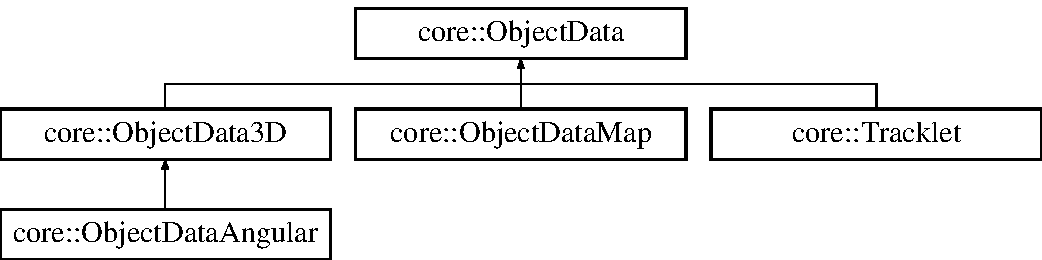
\includegraphics[height=2.000000cm]{classcore_1_1ObjectData}
\end{center}
\end{figure}
\subsection*{Public Member Functions}
\begin{DoxyCompactItemize}
\item 
\hyperlink{classcore_1_1ObjectData_a7f47a396a3b9e8c12a1557c8156b8ff9}{Object\+Data} ()
\item 
\hyperlink{classcore_1_1ObjectData_af4333a52b012841a6ba73b25aeaae71b}{Object\+Data} (std\+::size\+\_\+t frame\+\_\+index)
\item 
std\+::size\+\_\+t \hyperlink{classcore_1_1ObjectData_a1151e9215baf315f4b98f696f4271162}{Get\+Frame\+Index} () const
\item 
bool \hyperlink{classcore_1_1ObjectData_a2880d710cfa520e9c0453e2a6729c0e2}{Is\+Virtual} () const
\item 
virtual double \hyperlink{classcore_1_1ObjectData_a01f04d64b1e62f567d819a8fcbe38319}{Compare\+To} (\hyperlink{classcore_1_1ObjectData}{Object\+Data} $\ast$obj)
\end{DoxyCompactItemize}
\subsection*{Protected Member Functions}
\begin{DoxyCompactItemize}
\item 
virtual void \hyperlink{classcore_1_1ObjectData_aa26949b0456068d67802d9f6067aa657}{Print} (std\+::ostream \&os) const
\end{DoxyCompactItemize}
\subsection*{Protected Attributes}
\begin{DoxyCompactItemize}
\item 
std\+::size\+\_\+t \hyperlink{classcore_1_1ObjectData_ade1423dbad9323431d22750121fa59e5}{frame\+\_\+index\+\_\+}
\end{DoxyCompactItemize}
\subsection*{Friends}
\begin{DoxyCompactItemize}
\item 
std\+::ostream \& \hyperlink{classcore_1_1ObjectData_a56fc9b6184428bf4d80826bbb9fe4c6f}{operator$<$$<$} (std\+::ostream \&os, const \hyperlink{classcore_1_1ObjectData}{Object\+Data} \&obj)
\end{DoxyCompactItemize}


\subsection{Detailed Description}
Base class for all detected objects. Stores the corresponding frame index. 

\subsection{Constructor \& Destructor Documentation}
\index{core\+::\+Object\+Data@{core\+::\+Object\+Data}!Object\+Data@{Object\+Data}}
\index{Object\+Data@{Object\+Data}!core\+::\+Object\+Data@{core\+::\+Object\+Data}}
\subsubsection[{\texorpdfstring{Object\+Data()}{ObjectData()}}]{\setlength{\rightskip}{0pt plus 5cm}core\+::\+Object\+Data\+::\+Object\+Data (
\begin{DoxyParamCaption}
{}
\end{DoxyParamCaption}
)}\hypertarget{classcore_1_1ObjectData_a7f47a396a3b9e8c12a1557c8156b8ff9}{}\label{classcore_1_1ObjectData_a7f47a396a3b9e8c12a1557c8156b8ff9}
Creates a new empty \hyperlink{classcore_1_1ObjectData}{Object\+Data} (e.\+g. for virtual objects) \index{core\+::\+Object\+Data@{core\+::\+Object\+Data}!Object\+Data@{Object\+Data}}
\index{Object\+Data@{Object\+Data}!core\+::\+Object\+Data@{core\+::\+Object\+Data}}
\subsubsection[{\texorpdfstring{Object\+Data(std\+::size\+\_\+t frame\+\_\+index)}{ObjectData(std::size\_t frame\_index)}}]{\setlength{\rightskip}{0pt plus 5cm}core\+::\+Object\+Data\+::\+Object\+Data (
\begin{DoxyParamCaption}
\item[{std\+::size\+\_\+t}]{frame\+\_\+index}
\end{DoxyParamCaption}
)}\hypertarget{classcore_1_1ObjectData_af4333a52b012841a6ba73b25aeaae71b}{}\label{classcore_1_1ObjectData_af4333a52b012841a6ba73b25aeaae71b}
Creates a new \hyperlink{classcore_1_1ObjectData}{Object\+Data} with the given frame index 
\begin{DoxyParams}{Parameters}
{\em frame\+\_\+index} & the index in which the object was detected \\
\hline
\end{DoxyParams}


\subsection{Member Function Documentation}
\index{core\+::\+Object\+Data@{core\+::\+Object\+Data}!Compare\+To@{Compare\+To}}
\index{Compare\+To@{Compare\+To}!core\+::\+Object\+Data@{core\+::\+Object\+Data}}
\subsubsection[{\texorpdfstring{Compare\+To(\+Object\+Data $\ast$obj)}{CompareTo(ObjectData *obj)}}]{\setlength{\rightskip}{0pt plus 5cm}double core\+::\+Object\+Data\+::\+Compare\+To (
\begin{DoxyParamCaption}
\item[{{\bf Object\+Data} $\ast$}]{obj}
\end{DoxyParamCaption}
)\hspace{0.3cm}{\ttfamily [virtual]}}\hypertarget{classcore_1_1ObjectData_a01f04d64b1e62f567d819a8fcbe38319}{}\label{classcore_1_1ObjectData_a01f04d64b1e62f567d819a8fcbe38319}
Compares this object with the given object. 
\begin{DoxyParams}{Parameters}
{\em obj} & A pointer to the object to compare this object to \\
\hline
\end{DoxyParams}
\begin{DoxyReturn}{Returns}
A double value indicating the comparison result 
\end{DoxyReturn}


Reimplemented in \hyperlink{classcore_1_1ObjectDataMap_ad00d1998652e4d2ffa2629128c9c2947}{core\+::\+Object\+Data\+Map}, and \hyperlink{classcore_1_1Tracklet_ab45f28ba6abde0944820ac614560ea89}{core\+::\+Tracklet}.

\index{core\+::\+Object\+Data@{core\+::\+Object\+Data}!Get\+Frame\+Index@{Get\+Frame\+Index}}
\index{Get\+Frame\+Index@{Get\+Frame\+Index}!core\+::\+Object\+Data@{core\+::\+Object\+Data}}
\subsubsection[{\texorpdfstring{Get\+Frame\+Index() const}{GetFrameIndex() const}}]{\setlength{\rightskip}{0pt plus 5cm}std\+::size\+\_\+t core\+::\+Object\+Data\+::\+Get\+Frame\+Index (
\begin{DoxyParamCaption}
{}
\end{DoxyParamCaption}
) const}\hypertarget{classcore_1_1ObjectData_a1151e9215baf315f4b98f696f4271162}{}\label{classcore_1_1ObjectData_a1151e9215baf315f4b98f696f4271162}
Getter for the frame index \begin{DoxyReturn}{Returns}
The frame index 
\end{DoxyReturn}
\index{core\+::\+Object\+Data@{core\+::\+Object\+Data}!Is\+Virtual@{Is\+Virtual}}
\index{Is\+Virtual@{Is\+Virtual}!core\+::\+Object\+Data@{core\+::\+Object\+Data}}
\subsubsection[{\texorpdfstring{Is\+Virtual() const}{IsVirtual() const}}]{\setlength{\rightskip}{0pt plus 5cm}bool core\+::\+Object\+Data\+::\+Is\+Virtual (
\begin{DoxyParamCaption}
{}
\end{DoxyParamCaption}
) const}\hypertarget{classcore_1_1ObjectData_a2880d710cfa520e9c0453e2a6729c0e2}{}\label{classcore_1_1ObjectData_a2880d710cfa520e9c0453e2a6729c0e2}
Is this node considered a virtual node \begin{DoxyReturn}{Returns}
Whether this node is virtual 
\end{DoxyReturn}
\index{core\+::\+Object\+Data@{core\+::\+Object\+Data}!Print@{Print}}
\index{Print@{Print}!core\+::\+Object\+Data@{core\+::\+Object\+Data}}
\subsubsection[{\texorpdfstring{Print(std\+::ostream \&os) const}{Print(std::ostream \&os) const}}]{\setlength{\rightskip}{0pt plus 5cm}void core\+::\+Object\+Data\+::\+Print (
\begin{DoxyParamCaption}
\item[{std\+::ostream \&}]{os}
\end{DoxyParamCaption}
) const\hspace{0.3cm}{\ttfamily [protected]}, {\ttfamily [virtual]}}\hypertarget{classcore_1_1ObjectData_aa26949b0456068d67802d9f6067aa657}{}\label{classcore_1_1ObjectData_aa26949b0456068d67802d9f6067aa657}
Used in the $<$$<$ operator 
\begin{DoxyParams}{Parameters}
{\em os} & The stream to write to \\
\hline
\end{DoxyParams}


Reimplemented in \hyperlink{classcore_1_1ObjectDataMap_a16fbcc2b99feb1545e1a66f828680b1a}{core\+::\+Object\+Data\+Map}.



\subsection{Friends And Related Function Documentation}
\index{core\+::\+Object\+Data@{core\+::\+Object\+Data}!operator$<$$<$@{operator$<$$<$}}
\index{operator$<$$<$@{operator$<$$<$}!core\+::\+Object\+Data@{core\+::\+Object\+Data}}
\subsubsection[{\texorpdfstring{operator$<$$<$}{operator<<}}]{\setlength{\rightskip}{0pt plus 5cm}std\+::ostream\& operator$<$$<$ (
\begin{DoxyParamCaption}
\item[{std\+::ostream \&}]{os, }
\item[{const {\bf Object\+Data} \&}]{obj}
\end{DoxyParamCaption}
)\hspace{0.3cm}{\ttfamily [friend]}}\hypertarget{classcore_1_1ObjectData_a56fc9b6184428bf4d80826bbb9fe4c6f}{}\label{classcore_1_1ObjectData_a56fc9b6184428bf4d80826bbb9fe4c6f}
Overrides the $<$$<$ operator for easy output. Calls the print method. 
\begin{DoxyParams}{Parameters}
{\em os} & The stream to write to \\
\hline
{\em obj} & The object to write into the stream \\
\hline
\end{DoxyParams}
\begin{DoxyReturn}{Returns}
The stream written to 
\end{DoxyReturn}


\subsection{Member Data Documentation}
\index{core\+::\+Object\+Data@{core\+::\+Object\+Data}!frame\+\_\+index\+\_\+@{frame\+\_\+index\+\_\+}}
\index{frame\+\_\+index\+\_\+@{frame\+\_\+index\+\_\+}!core\+::\+Object\+Data@{core\+::\+Object\+Data}}
\subsubsection[{\texorpdfstring{frame\+\_\+index\+\_\+}{frame\_index\_}}]{\setlength{\rightskip}{0pt plus 5cm}std\+::size\+\_\+t core\+::\+Object\+Data\+::frame\+\_\+index\+\_\+\hspace{0.3cm}{\ttfamily [protected]}}\hypertarget{classcore_1_1ObjectData_ade1423dbad9323431d22750121fa59e5}{}\label{classcore_1_1ObjectData_ade1423dbad9323431d22750121fa59e5}
The frame the object was detected in 

The documentation for this class was generated from the following files\+:\begin{DoxyCompactItemize}
\item 
core/Object\+Data.\+h\item 
core/Object\+Data.\+cpp\end{DoxyCompactItemize}

\hypertarget{classcore_1_1ObjectData3D}{}\section{core\+:\+:Object\+Data3D Class Reference}
\label{classcore_1_1ObjectData3D}\index{core\+::\+Object\+Data3D@{core\+::\+Object\+Data3D}}


{\ttfamily \#include $<$Object\+Data3\+D.\+h$>$}

Inheritance diagram for core\+:\+:Object\+Data3D\+:\begin{figure}[H]
\begin{center}
\leavevmode
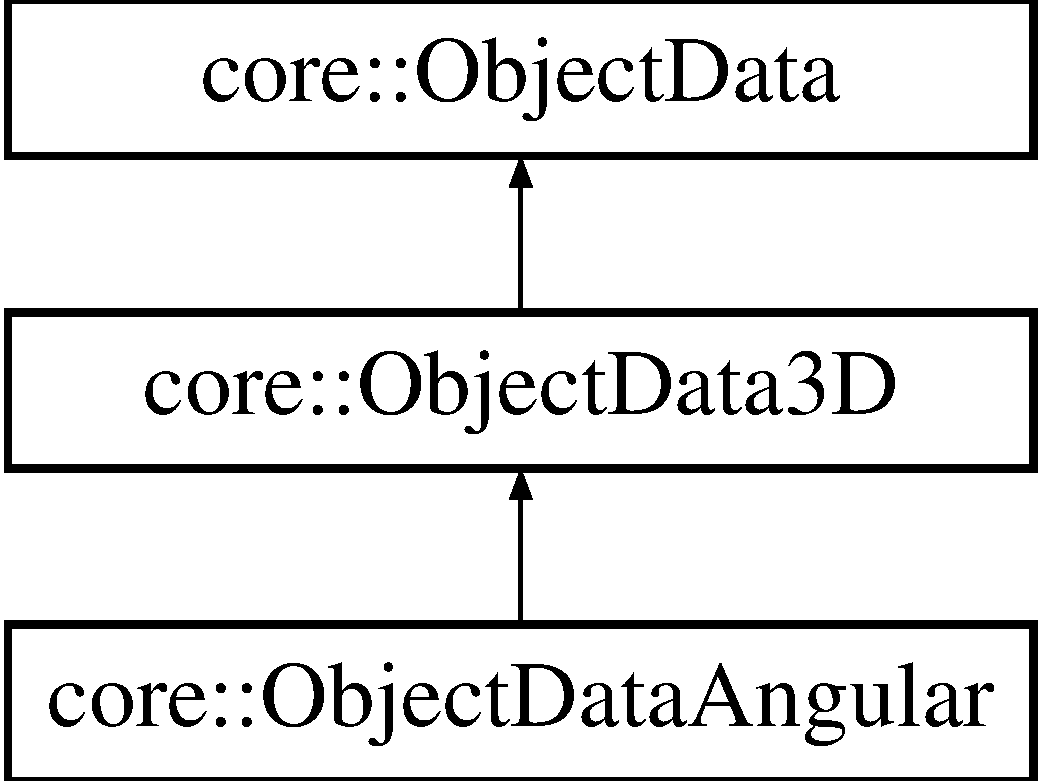
\includegraphics[height=3.000000cm]{classcore_1_1ObjectData3D}
\end{center}
\end{figure}
\subsection*{Public Member Functions}
\begin{DoxyCompactItemize}
\item 
\hyperlink{classcore_1_1ObjectData3D_a47c967cffcbd109f1366069958a71699}{Object\+Data3D} (size\+\_\+t frame\+\_\+index, cv\+::\+Point3d position)
\item 
void \hyperlink{classcore_1_1ObjectData3D_a05eafbd4d963ef14b1068ab5a3818597}{Set\+Temporal\+Weight} (double weight)
\item 
void \hyperlink{classcore_1_1ObjectData3D_a94d4c0d90d4e0999eb2b339d37069cd6}{Set\+Spatial\+Weight} (double weight)
\item 
cv\+::\+Point3d \hyperlink{classcore_1_1ObjectData3D_a0f4a0dca51eb50fdc5baf9714c4a64f6}{Get\+Position} () const
\item 
double \hyperlink{classcore_1_1ObjectData3D_a155e3f4dd2a6adb5d32b61f224092d4b}{Get\+Temporal\+Weight} () const
\item 
double \hyperlink{classcore_1_1ObjectData3D_a896607721c9d12b2e2425fe927f06d6f}{Get\+Spatial\+Weight} () const
\item 
virtual double \hyperlink{classcore_1_1ObjectData3D_abef3e4e7a0dc121d8a403d91964be576}{Compare\+To} (Object\+Data\+Ptr obj) const override
\item 
virtual Object\+Data\+Ptr \hyperlink{classcore_1_1ObjectData3D_ae57a5d8f7a02a403653c82c3b73a73d2}{Interpolate} (Object\+Data\+Ptr obj, double fraction) const override
\item 
virtual void \hyperlink{classcore_1_1ObjectData3D_a86216fae3dc86f1107eb1b4530b574d2}{Visualize} (cv\+::\+Mat \&image, cv\+::\+Scalar \&color) const override
\end{DoxyCompactItemize}


\subsection{Detailed Description}
Class for storing a detection in three dimensional space. 

\subsection{Constructor \& Destructor Documentation}
\index{core\+::\+Object\+Data3D@{core\+::\+Object\+Data3D}!Object\+Data3D@{Object\+Data3D}}
\index{Object\+Data3D@{Object\+Data3D}!core\+::\+Object\+Data3D@{core\+::\+Object\+Data3D}}
\subsubsection[{\texorpdfstring{Object\+Data3\+D(size\+\_\+t frame\+\_\+index, cv\+::\+Point3d position)}{ObjectData3D(size\_t frame\_index, cv::Point3d position)}}]{\setlength{\rightskip}{0pt plus 5cm}core\+::\+Object\+Data3\+D\+::\+Object\+Data3D (
\begin{DoxyParamCaption}
\item[{size\+\_\+t}]{frame\+\_\+index, }
\item[{cv\+::\+Point3d}]{position}
\end{DoxyParamCaption}
)}\hypertarget{classcore_1_1ObjectData3D_a47c967cffcbd109f1366069958a71699}{}\label{classcore_1_1ObjectData3D_a47c967cffcbd109f1366069958a71699}
Creates a new detection with the given index and position. 
\begin{DoxyParams}{Parameters}
{\em frame\+\_\+index} & The frame index \\
\hline
{\em position} & The position in three dimensional space \\
\hline
\end{DoxyParams}


\subsection{Member Function Documentation}
\index{core\+::\+Object\+Data3D@{core\+::\+Object\+Data3D}!Compare\+To@{Compare\+To}}
\index{Compare\+To@{Compare\+To}!core\+::\+Object\+Data3D@{core\+::\+Object\+Data3D}}
\subsubsection[{\texorpdfstring{Compare\+To(\+Object\+Data\+Ptr obj) const override}{CompareTo(ObjectDataPtr obj) const override}}]{\setlength{\rightskip}{0pt plus 5cm}double core\+::\+Object\+Data3\+D\+::\+Compare\+To (
\begin{DoxyParamCaption}
\item[{Object\+Data\+Ptr}]{obj}
\end{DoxyParamCaption}
) const\hspace{0.3cm}{\ttfamily [override]}, {\ttfamily [virtual]}}\hypertarget{classcore_1_1ObjectData3D_abef3e4e7a0dc121d8a403d91964be576}{}\label{classcore_1_1ObjectData3D_abef3e4e7a0dc121d8a403d91964be576}
Compares this object with the given object. 
\begin{DoxyParams}{Parameters}
{\em obj} & A pointer to the object to compare this object to \\
\hline
\end{DoxyParams}
\begin{DoxyReturn}{Returns}
A double value indicating the comparison result 
\end{DoxyReturn}


Reimplemented from \hyperlink{classcore_1_1ObjectData_afbf7a1e87235f1b204d4d2eb8a37a9a6}{core\+::\+Object\+Data}.



Reimplemented in \hyperlink{classcore_1_1ObjectDataAngular_a2932240c6c082b76f2c04723cdf3e4f9}{core\+::\+Object\+Data\+Angular}.

\index{core\+::\+Object\+Data3D@{core\+::\+Object\+Data3D}!Get\+Position@{Get\+Position}}
\index{Get\+Position@{Get\+Position}!core\+::\+Object\+Data3D@{core\+::\+Object\+Data3D}}
\subsubsection[{\texorpdfstring{Get\+Position() const}{GetPosition() const}}]{\setlength{\rightskip}{0pt plus 5cm}cv\+::\+Point3d core\+::\+Object\+Data3\+D\+::\+Get\+Position (
\begin{DoxyParamCaption}
{}
\end{DoxyParamCaption}
) const}\hypertarget{classcore_1_1ObjectData3D_a0f4a0dca51eb50fdc5baf9714c4a64f6}{}\label{classcore_1_1ObjectData3D_a0f4a0dca51eb50fdc5baf9714c4a64f6}
Gets the position in three dimensional space. \begin{DoxyReturn}{Returns}
The position 
\end{DoxyReturn}
\index{core\+::\+Object\+Data3D@{core\+::\+Object\+Data3D}!Get\+Spatial\+Weight@{Get\+Spatial\+Weight}}
\index{Get\+Spatial\+Weight@{Get\+Spatial\+Weight}!core\+::\+Object\+Data3D@{core\+::\+Object\+Data3D}}
\subsubsection[{\texorpdfstring{Get\+Spatial\+Weight() const}{GetSpatialWeight() const}}]{\setlength{\rightskip}{0pt plus 5cm}double core\+::\+Object\+Data3\+D\+::\+Get\+Spatial\+Weight (
\begin{DoxyParamCaption}
{}
\end{DoxyParamCaption}
) const}\hypertarget{classcore_1_1ObjectData3D_a896607721c9d12b2e2425fe927f06d6f}{}\label{classcore_1_1ObjectData3D_a896607721c9d12b2e2425fe927f06d6f}
Gets the spatial weight \begin{DoxyReturn}{Returns}
The spatial weight 
\end{DoxyReturn}
\index{core\+::\+Object\+Data3D@{core\+::\+Object\+Data3D}!Get\+Temporal\+Weight@{Get\+Temporal\+Weight}}
\index{Get\+Temporal\+Weight@{Get\+Temporal\+Weight}!core\+::\+Object\+Data3D@{core\+::\+Object\+Data3D}}
\subsubsection[{\texorpdfstring{Get\+Temporal\+Weight() const}{GetTemporalWeight() const}}]{\setlength{\rightskip}{0pt plus 5cm}double core\+::\+Object\+Data3\+D\+::\+Get\+Temporal\+Weight (
\begin{DoxyParamCaption}
{}
\end{DoxyParamCaption}
) const}\hypertarget{classcore_1_1ObjectData3D_a155e3f4dd2a6adb5d32b61f224092d4b}{}\label{classcore_1_1ObjectData3D_a155e3f4dd2a6adb5d32b61f224092d4b}
Gets the temporal weight. \begin{DoxyReturn}{Returns}
The temporal weight 
\end{DoxyReturn}
\index{core\+::\+Object\+Data3D@{core\+::\+Object\+Data3D}!Interpolate@{Interpolate}}
\index{Interpolate@{Interpolate}!core\+::\+Object\+Data3D@{core\+::\+Object\+Data3D}}
\subsubsection[{\texorpdfstring{Interpolate(\+Object\+Data\+Ptr obj, double fraction) const override}{Interpolate(ObjectDataPtr obj, double fraction) const override}}]{\setlength{\rightskip}{0pt plus 5cm}Object\+Data\+Ptr core\+::\+Object\+Data3\+D\+::\+Interpolate (
\begin{DoxyParamCaption}
\item[{Object\+Data\+Ptr}]{obj, }
\item[{double}]{fraction}
\end{DoxyParamCaption}
) const\hspace{0.3cm}{\ttfamily [override]}, {\ttfamily [virtual]}}\hypertarget{classcore_1_1ObjectData3D_ae57a5d8f7a02a403653c82c3b73a73d2}{}\label{classcore_1_1ObjectData3D_ae57a5d8f7a02a403653c82c3b73a73d2}
Linearly interpolates between this and the given object. Creates a new object to fit between the two objects. 
\begin{DoxyParams}{Parameters}
{\em obj} & A pointer to the target object \\
\hline
{\em fraction} & Describes where the interpolation should be done. A fraction of zero is a clone of this object, a fraction of one is a clone of the target object. \\
\hline
\end{DoxyParams}
\begin{DoxyReturn}{Returns}
The interpolated object 
\end{DoxyReturn}


Reimplemented from \hyperlink{classcore_1_1ObjectData_ad681915317decab76c384a635fc8444e}{core\+::\+Object\+Data}.



Reimplemented in \hyperlink{classcore_1_1ObjectDataAngular_a42962dd1f994b2577133450e755d586e}{core\+::\+Object\+Data\+Angular}.

\index{core\+::\+Object\+Data3D@{core\+::\+Object\+Data3D}!Set\+Spatial\+Weight@{Set\+Spatial\+Weight}}
\index{Set\+Spatial\+Weight@{Set\+Spatial\+Weight}!core\+::\+Object\+Data3D@{core\+::\+Object\+Data3D}}
\subsubsection[{\texorpdfstring{Set\+Spatial\+Weight(double weight)}{SetSpatialWeight(double weight)}}]{\setlength{\rightskip}{0pt plus 5cm}void core\+::\+Object\+Data3\+D\+::\+Set\+Spatial\+Weight (
\begin{DoxyParamCaption}
\item[{double}]{weight}
\end{DoxyParamCaption}
)}\hypertarget{classcore_1_1ObjectData3D_a94d4c0d90d4e0999eb2b339d37069cd6}{}\label{classcore_1_1ObjectData3D_a94d4c0d90d4e0999eb2b339d37069cd6}
Sets the spatial weight 
\begin{DoxyParams}{Parameters}
{\em weight} & The spatial weight \\
\hline
\end{DoxyParams}
\index{core\+::\+Object\+Data3D@{core\+::\+Object\+Data3D}!Set\+Temporal\+Weight@{Set\+Temporal\+Weight}}
\index{Set\+Temporal\+Weight@{Set\+Temporal\+Weight}!core\+::\+Object\+Data3D@{core\+::\+Object\+Data3D}}
\subsubsection[{\texorpdfstring{Set\+Temporal\+Weight(double weight)}{SetTemporalWeight(double weight)}}]{\setlength{\rightskip}{0pt plus 5cm}void core\+::\+Object\+Data3\+D\+::\+Set\+Temporal\+Weight (
\begin{DoxyParamCaption}
\item[{double}]{weight}
\end{DoxyParamCaption}
)}\hypertarget{classcore_1_1ObjectData3D_a05eafbd4d963ef14b1068ab5a3818597}{}\label{classcore_1_1ObjectData3D_a05eafbd4d963ef14b1068ab5a3818597}
Sets the temporal weight. 
\begin{DoxyParams}{Parameters}
{\em weight} & The temporal weight \\
\hline
\end{DoxyParams}
\index{core\+::\+Object\+Data3D@{core\+::\+Object\+Data3D}!Visualize@{Visualize}}
\index{Visualize@{Visualize}!core\+::\+Object\+Data3D@{core\+::\+Object\+Data3D}}
\subsubsection[{\texorpdfstring{Visualize(cv\+::\+Mat \&image, cv\+::\+Scalar \&color) const override}{Visualize(cv::Mat \&image, cv::Scalar \&color) const override}}]{\setlength{\rightskip}{0pt plus 5cm}void core\+::\+Object\+Data3\+D\+::\+Visualize (
\begin{DoxyParamCaption}
\item[{cv\+::\+Mat \&}]{image, }
\item[{cv\+::\+Scalar \&}]{color}
\end{DoxyParamCaption}
) const\hspace{0.3cm}{\ttfamily [override]}, {\ttfamily [virtual]}}\hypertarget{classcore_1_1ObjectData3D_a86216fae3dc86f1107eb1b4530b574d2}{}\label{classcore_1_1ObjectData3D_a86216fae3dc86f1107eb1b4530b574d2}
Visualizes the object in the given image with the given color. This method does nothing, it needs to be overwritten to visualize something. 
\begin{DoxyParams}{Parameters}
{\em image} & The image to write into \\
\hline
{\em color} & The color to use \\
\hline
\end{DoxyParams}


Reimplemented from \hyperlink{classcore_1_1ObjectData_aae2c4fceddc529570dbe8909309f9961}{core\+::\+Object\+Data}.



Reimplemented in \hyperlink{classcore_1_1ObjectDataAngular_acb4265f6de511238460df118148bc85c}{core\+::\+Object\+Data\+Angular}.



The documentation for this class was generated from the following files\+:\begin{DoxyCompactItemize}
\item 
core/Object\+Data3\+D.\+h\item 
core/Object\+Data3\+D.\+cpp\end{DoxyCompactItemize}

\hypertarget{classcore_1_1ObjectDataAngular}{}\section{core\+:\+:Object\+Data\+Angular Class Reference}
\label{classcore_1_1ObjectDataAngular}\index{core\+::\+Object\+Data\+Angular@{core\+::\+Object\+Data\+Angular}}


{\ttfamily \#include $<$Object\+Data\+Angular.\+h$>$}

Inheritance diagram for core\+:\+:Object\+Data\+Angular\+:\begin{figure}[H]
\begin{center}
\leavevmode
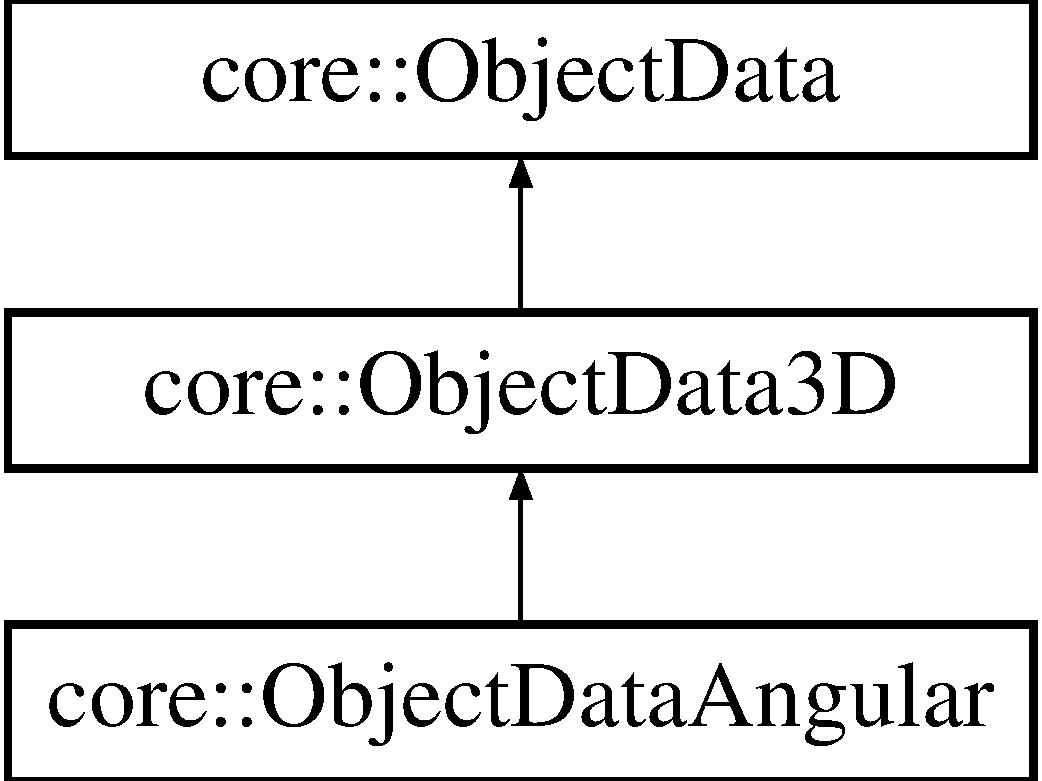
\includegraphics[height=3.000000cm]{classcore_1_1ObjectDataAngular}
\end{center}
\end{figure}
\subsection*{Public Member Functions}
\begin{DoxyCompactItemize}
\item 
\hyperlink{classcore_1_1ObjectDataAngular_a276b02fc7646e3275f1cb81fca7e9a47}{Object\+Data\+Angular} (size\+\_\+t frame\+\_\+index, const cv\+::\+Point2d \&position, double angle)
\item 
\hyperlink{classcore_1_1ObjectDataAngular_aae3a8f335e26771d06c8940931d5d654}{Object\+Data\+Angular} (size\+\_\+t frame\+\_\+index, const cv\+::\+Point2d \&position, double angle, double temporal\+\_\+weight, double spatial\+\_\+weight, double angular\+\_\+weight)
\item 
void \hyperlink{classcore_1_1ObjectDataAngular_af6772caef2337f3c12a3f52049c4d853}{Set\+Angular\+Weight} (double weight)
\item 
double \hyperlink{classcore_1_1ObjectDataAngular_a6c2da5010cd919af3b0f156579d04ef8}{Get\+Angle} () const
\item 
double \hyperlink{classcore_1_1ObjectDataAngular_ae1c5db7b9fc06e648450d9388c93a1aa}{Get\+Angular\+Weight} () const
\item 
virtual double \hyperlink{classcore_1_1ObjectDataAngular_a2932240c6c082b76f2c04723cdf3e4f9}{Compare\+To} (Object\+Data\+Ptr obj) const override
\item 
virtual bool \hyperlink{classcore_1_1ObjectDataAngular_a1ef9168c2384d2038a1dd6e85d0b932f}{Is\+Within\+Constraints} (Object\+Data\+Ptr obj, std\+::unordered\+\_\+map$<$ std\+::string, double $>$ \&constraints) const override
\item 
virtual Object\+Data\+Ptr \hyperlink{classcore_1_1ObjectDataAngular_a42962dd1f994b2577133450e755d586e}{Interpolate} (Object\+Data\+Ptr obj, double fraction) const override
\item 
virtual void \hyperlink{classcore_1_1ObjectDataAngular_acb4265f6de511238460df118148bc85c}{Visualize} (cv\+::\+Mat \&image, cv\+::\+Scalar \&color) const override
\item 
virtual std\+::string \hyperlink{classcore_1_1ObjectDataAngular_a3b419c1d4be886f094b9af94cd839bd4}{To\+String} (char delimiter) const override
\end{DoxyCompactItemize}


\subsection{Detailed Description}
Class for storing a detection in two dimensional space with an rotation angle in radians. 

\subsection{Constructor \& Destructor Documentation}
\index{core\+::\+Object\+Data\+Angular@{core\+::\+Object\+Data\+Angular}!Object\+Data\+Angular@{Object\+Data\+Angular}}
\index{Object\+Data\+Angular@{Object\+Data\+Angular}!core\+::\+Object\+Data\+Angular@{core\+::\+Object\+Data\+Angular}}
\subsubsection[{\texorpdfstring{Object\+Data\+Angular(size\+\_\+t frame\+\_\+index, const cv\+::\+Point2d \&position, double angle)}{ObjectDataAngular(size\_t frame\_index, const cv::Point2d \&position, double angle)}}]{\setlength{\rightskip}{0pt plus 5cm}core\+::\+Object\+Data\+Angular\+::\+Object\+Data\+Angular (
\begin{DoxyParamCaption}
\item[{size\+\_\+t}]{frame\+\_\+index, }
\item[{const cv\+::\+Point2d \&}]{position, }
\item[{double}]{angle}
\end{DoxyParamCaption}
)}\hypertarget{classcore_1_1ObjectDataAngular_a276b02fc7646e3275f1cb81fca7e9a47}{}\label{classcore_1_1ObjectDataAngular_a276b02fc7646e3275f1cb81fca7e9a47}
Creates a new object in the given frame, with the given position and the given angle. 
\begin{DoxyParams}{Parameters}
{\em frame\+\_\+index} & The index of the frame \\
\hline
{\em position} & The position in two dimensional space \\
\hline
{\em angle} & The rotation angle in radians \\
\hline
\end{DoxyParams}
\index{core\+::\+Object\+Data\+Angular@{core\+::\+Object\+Data\+Angular}!Object\+Data\+Angular@{Object\+Data\+Angular}}
\index{Object\+Data\+Angular@{Object\+Data\+Angular}!core\+::\+Object\+Data\+Angular@{core\+::\+Object\+Data\+Angular}}
\subsubsection[{\texorpdfstring{Object\+Data\+Angular(size\+\_\+t frame\+\_\+index, const cv\+::\+Point2d \&position, double angle, double temporal\+\_\+weight, double spatial\+\_\+weight, double angular\+\_\+weight)}{ObjectDataAngular(size\_t frame\_index, const cv::Point2d \&position, double angle, double temporal\_weight, double spatial\_weight, double angular\_weight)}}]{\setlength{\rightskip}{0pt plus 5cm}core\+::\+Object\+Data\+Angular\+::\+Object\+Data\+Angular (
\begin{DoxyParamCaption}
\item[{size\+\_\+t}]{frame\+\_\+index, }
\item[{const cv\+::\+Point2d \&}]{position, }
\item[{double}]{angle, }
\item[{double}]{temporal\+\_\+weight, }
\item[{double}]{spatial\+\_\+weight, }
\item[{double}]{angular\+\_\+weight}
\end{DoxyParamCaption}
)}\hypertarget{classcore_1_1ObjectDataAngular_aae3a8f335e26771d06c8940931d5d654}{}\label{classcore_1_1ObjectDataAngular_aae3a8f335e26771d06c8940931d5d654}
Creates a new object in the given frame, with the given position and the given angle. The weights are used in the comparison calculation. 
\begin{DoxyParams}{Parameters}
{\em frame\+\_\+index} & The index of the frame \\
\hline
{\em position} & The position in two dimensional space \\
\hline
{\em angle} & The rotation angle in radians \\
\hline
{\em temporal\+\_\+weight} & The temporal weight \\
\hline
{\em spatial\+\_\+weight} & The spatial weight \\
\hline
{\em angular\+\_\+weight} & The angular weight \\
\hline
\end{DoxyParams}


\subsection{Member Function Documentation}
\index{core\+::\+Object\+Data\+Angular@{core\+::\+Object\+Data\+Angular}!Compare\+To@{Compare\+To}}
\index{Compare\+To@{Compare\+To}!core\+::\+Object\+Data\+Angular@{core\+::\+Object\+Data\+Angular}}
\subsubsection[{\texorpdfstring{Compare\+To(\+Object\+Data\+Ptr obj) const override}{CompareTo(ObjectDataPtr obj) const override}}]{\setlength{\rightskip}{0pt plus 5cm}double core\+::\+Object\+Data\+Angular\+::\+Compare\+To (
\begin{DoxyParamCaption}
\item[{Object\+Data\+Ptr}]{obj}
\end{DoxyParamCaption}
) const\hspace{0.3cm}{\ttfamily [override]}, {\ttfamily [virtual]}}\hypertarget{classcore_1_1ObjectDataAngular_a2932240c6c082b76f2c04723cdf3e4f9}{}\label{classcore_1_1ObjectDataAngular_a2932240c6c082b76f2c04723cdf3e4f9}
Compares this object with the given object. 
\begin{DoxyParams}{Parameters}
{\em obj} & A pointer to the object to compare this object to \\
\hline
\end{DoxyParams}
\begin{DoxyReturn}{Returns}
A double value indicating the comparison result 
\end{DoxyReturn}


Reimplemented from \hyperlink{classcore_1_1ObjectData2D_a68d56bd5f26a41830a87ae32eabf9126}{core\+::\+Object\+Data2D}.

\index{core\+::\+Object\+Data\+Angular@{core\+::\+Object\+Data\+Angular}!Get\+Angle@{Get\+Angle}}
\index{Get\+Angle@{Get\+Angle}!core\+::\+Object\+Data\+Angular@{core\+::\+Object\+Data\+Angular}}
\subsubsection[{\texorpdfstring{Get\+Angle() const}{GetAngle() const}}]{\setlength{\rightskip}{0pt plus 5cm}double core\+::\+Object\+Data\+Angular\+::\+Get\+Angle (
\begin{DoxyParamCaption}
{}
\end{DoxyParamCaption}
) const}\hypertarget{classcore_1_1ObjectDataAngular_a6c2da5010cd919af3b0f156579d04ef8}{}\label{classcore_1_1ObjectDataAngular_a6c2da5010cd919af3b0f156579d04ef8}
Gets the rotation angle in radians. \begin{DoxyReturn}{Returns}
The rotation angle in radians 
\end{DoxyReturn}
\index{core\+::\+Object\+Data\+Angular@{core\+::\+Object\+Data\+Angular}!Get\+Angular\+Weight@{Get\+Angular\+Weight}}
\index{Get\+Angular\+Weight@{Get\+Angular\+Weight}!core\+::\+Object\+Data\+Angular@{core\+::\+Object\+Data\+Angular}}
\subsubsection[{\texorpdfstring{Get\+Angular\+Weight() const}{GetAngularWeight() const}}]{\setlength{\rightskip}{0pt plus 5cm}double core\+::\+Object\+Data\+Angular\+::\+Get\+Angular\+Weight (
\begin{DoxyParamCaption}
{}
\end{DoxyParamCaption}
) const}\hypertarget{classcore_1_1ObjectDataAngular_ae1c5db7b9fc06e648450d9388c93a1aa}{}\label{classcore_1_1ObjectDataAngular_ae1c5db7b9fc06e648450d9388c93a1aa}
Gets the angular weight. \begin{DoxyReturn}{Returns}
The angular weight 
\end{DoxyReturn}
\index{core\+::\+Object\+Data\+Angular@{core\+::\+Object\+Data\+Angular}!Interpolate@{Interpolate}}
\index{Interpolate@{Interpolate}!core\+::\+Object\+Data\+Angular@{core\+::\+Object\+Data\+Angular}}
\subsubsection[{\texorpdfstring{Interpolate(\+Object\+Data\+Ptr obj, double fraction) const override}{Interpolate(ObjectDataPtr obj, double fraction) const override}}]{\setlength{\rightskip}{0pt plus 5cm}Object\+Data\+Ptr core\+::\+Object\+Data\+Angular\+::\+Interpolate (
\begin{DoxyParamCaption}
\item[{Object\+Data\+Ptr}]{obj, }
\item[{double}]{fraction}
\end{DoxyParamCaption}
) const\hspace{0.3cm}{\ttfamily [override]}, {\ttfamily [virtual]}}\hypertarget{classcore_1_1ObjectDataAngular_a42962dd1f994b2577133450e755d586e}{}\label{classcore_1_1ObjectDataAngular_a42962dd1f994b2577133450e755d586e}
Linearly interpolates between this and the given object. Creates a new object to fit between the two objects. 
\begin{DoxyParams}{Parameters}
{\em obj} & A pointer to the target object \\
\hline
{\em fraction} & Describes where the interpolation should be done. A fraction of zero is a clone of this object, a fraction of one is a clone of the target object. \\
\hline
\end{DoxyParams}
\begin{DoxyReturn}{Returns}
The interpolated object 
\end{DoxyReturn}


Reimplemented from \hyperlink{classcore_1_1ObjectData2D_a59b974e09f74f0a2640e3152893fe79f}{core\+::\+Object\+Data2D}.

\index{core\+::\+Object\+Data\+Angular@{core\+::\+Object\+Data\+Angular}!Is\+Within\+Constraints@{Is\+Within\+Constraints}}
\index{Is\+Within\+Constraints@{Is\+Within\+Constraints}!core\+::\+Object\+Data\+Angular@{core\+::\+Object\+Data\+Angular}}
\subsubsection[{\texorpdfstring{Is\+Within\+Constraints(\+Object\+Data\+Ptr obj, std\+::unordered\+\_\+map$<$ std\+::string, double $>$ \&constraints) const override}{IsWithinConstraints(ObjectDataPtr obj, std::unordered\_map< std::string, double > \&constraints) const override}}]{\setlength{\rightskip}{0pt plus 5cm}bool core\+::\+Object\+Data\+Angular\+::\+Is\+Within\+Constraints (
\begin{DoxyParamCaption}
\item[{Object\+Data\+Ptr}]{obj, }
\item[{std\+::unordered\+\_\+map$<$ std\+::string, double $>$ \&}]{constraints}
\end{DoxyParamCaption}
) const\hspace{0.3cm}{\ttfamily [override]}, {\ttfamily [virtual]}}\hypertarget{classcore_1_1ObjectDataAngular_a1ef9168c2384d2038a1dd6e85d0b932f}{}\label{classcore_1_1ObjectDataAngular_a1ef9168c2384d2038a1dd6e85d0b932f}
Checks if the difference between this object and the specified object is within the constraints specified. The difference is calculated for each constraint separately.


\begin{DoxyParams}{Parameters}
{\em obj} & The object to get the difference to \\
\hline
{\em constraints} & The constraints to assure \\
\hline
\end{DoxyParams}


Reimplemented from \hyperlink{classcore_1_1ObjectData2D_a63e855919a72462225a8e69140f1389b}{core\+::\+Object\+Data2D}.

\index{core\+::\+Object\+Data\+Angular@{core\+::\+Object\+Data\+Angular}!Set\+Angular\+Weight@{Set\+Angular\+Weight}}
\index{Set\+Angular\+Weight@{Set\+Angular\+Weight}!core\+::\+Object\+Data\+Angular@{core\+::\+Object\+Data\+Angular}}
\subsubsection[{\texorpdfstring{Set\+Angular\+Weight(double weight)}{SetAngularWeight(double weight)}}]{\setlength{\rightskip}{0pt plus 5cm}void core\+::\+Object\+Data\+Angular\+::\+Set\+Angular\+Weight (
\begin{DoxyParamCaption}
\item[{double}]{weight}
\end{DoxyParamCaption}
)}\hypertarget{classcore_1_1ObjectDataAngular_af6772caef2337f3c12a3f52049c4d853}{}\label{classcore_1_1ObjectDataAngular_af6772caef2337f3c12a3f52049c4d853}
Sets the angular weight. 
\begin{DoxyParams}{Parameters}
{\em weight} & The angular weight \\
\hline
\end{DoxyParams}
\index{core\+::\+Object\+Data\+Angular@{core\+::\+Object\+Data\+Angular}!To\+String@{To\+String}}
\index{To\+String@{To\+String}!core\+::\+Object\+Data\+Angular@{core\+::\+Object\+Data\+Angular}}
\subsubsection[{\texorpdfstring{To\+String(char delimiter) const override}{ToString(char delimiter) const override}}]{\setlength{\rightskip}{0pt plus 5cm}std\+::string core\+::\+Object\+Data\+Angular\+::\+To\+String (
\begin{DoxyParamCaption}
\item[{char}]{delimiter}
\end{DoxyParamCaption}
) const\hspace{0.3cm}{\ttfamily [override]}, {\ttfamily [virtual]}}\hypertarget{classcore_1_1ObjectDataAngular_a3b419c1d4be886f094b9af94cd839bd4}{}\label{classcore_1_1ObjectDataAngular_a3b419c1d4be886f094b9af94cd839bd4}
Returns a string representing the values of this object data.


\begin{DoxyParams}{Parameters}
{\em delimiter} & The delimiter used to separate values \\
\hline
\end{DoxyParams}
\begin{DoxyReturn}{Returns}
The string containing the values 
\end{DoxyReturn}


Reimplemented from \hyperlink{classcore_1_1ObjectData2D_a72b2f50ca82ebd9269e1c29cdac6d92a}{core\+::\+Object\+Data2D}.

\index{core\+::\+Object\+Data\+Angular@{core\+::\+Object\+Data\+Angular}!Visualize@{Visualize}}
\index{Visualize@{Visualize}!core\+::\+Object\+Data\+Angular@{core\+::\+Object\+Data\+Angular}}
\subsubsection[{\texorpdfstring{Visualize(cv\+::\+Mat \&image, cv\+::\+Scalar \&color) const override}{Visualize(cv::Mat \&image, cv::Scalar \&color) const override}}]{\setlength{\rightskip}{0pt plus 5cm}void core\+::\+Object\+Data\+Angular\+::\+Visualize (
\begin{DoxyParamCaption}
\item[{cv\+::\+Mat \&}]{image, }
\item[{cv\+::\+Scalar \&}]{color}
\end{DoxyParamCaption}
) const\hspace{0.3cm}{\ttfamily [override]}, {\ttfamily [virtual]}}\hypertarget{classcore_1_1ObjectDataAngular_acb4265f6de511238460df118148bc85c}{}\label{classcore_1_1ObjectDataAngular_acb4265f6de511238460df118148bc85c}
Visualizes the object in the given image with the given color. This method does nothing, it needs to be overwritten to visualize something. 
\begin{DoxyParams}{Parameters}
{\em image} & The image to write into \\
\hline
{\em color} & The color to use \\
\hline
\end{DoxyParams}


Reimplemented from \hyperlink{classcore_1_1ObjectData2D_aff4e8539559f4ce50a7f43b733d6c512}{core\+::\+Object\+Data2D}.



The documentation for this class was generated from the following files\+:\begin{DoxyCompactItemize}
\item 
core/Object\+Data\+Angular.\+h\item 
core/Object\+Data\+Angular.\+cpp\end{DoxyCompactItemize}

\hypertarget{classcore_1_1ObjectDataMap}{}\section{core\+:\+:Object\+Data\+Map Class Reference}
\label{classcore_1_1ObjectDataMap}\index{core\+::\+Object\+Data\+Map@{core\+::\+Object\+Data\+Map}}


{\ttfamily \#include $<$Object\+Data\+Map.\+h$>$}

Inheritance diagram for core\+:\+:Object\+Data\+Map\+:\begin{figure}[H]
\begin{center}
\leavevmode
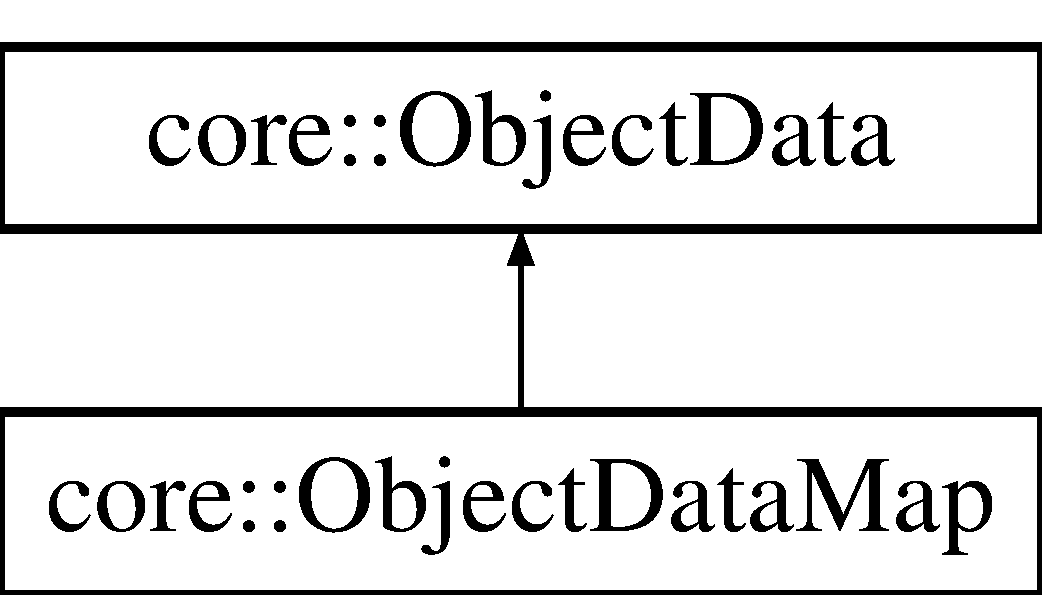
\includegraphics[height=2.000000cm]{classcore_1_1ObjectDataMap}
\end{center}
\end{figure}
\subsection*{Public Member Functions}
\begin{DoxyCompactItemize}
\item 
\hyperlink{classcore_1_1ObjectDataMap_ac6df34682a715db6845667f7dda1c795}{Object\+Data\+Map} (size\+\_\+t frame\+\_\+index)
\item 
\hyperlink{classcore_1_1ObjectDataMap_a573add8d73646e6c5f183a9a0c159596}{Object\+Data\+Map} (size\+\_\+t frame\+\_\+index, std\+::vector$<$ std\+::string $>$ keys, std\+::vector$<$ double $>$ value\+\_\+list)
\item 
\hyperlink{classcore_1_1ObjectDataMap_a5727c237d73f3f16c94a748c1b9b0c74}{Object\+Data\+Map} (size\+\_\+t frame\+\_\+index, std\+::vector$<$ std\+::string $>$ keys, std\+::vector$<$ double $>$ value\+\_\+list, std\+::vector$<$ double $>$ weight\+\_\+list)
\item 
\hyperlink{classcore_1_1ObjectDataMap_ad2af0de7438ed72be68348ac992568b6}{Object\+Data\+Map} (size\+\_\+t frame\+\_\+index, std\+::vector$<$ std\+::string $>$ keys, std\+::vector$<$ std\+::pair$<$ double, double $>$$>$ value\+\_\+weight\+\_\+list)
\item 
double \hyperlink{classcore_1_1ObjectDataMap_a276c89da6f3318d2baa2e9678e9508f7}{Get\+Value} (std\+::string key)
\item 
double \hyperlink{classcore_1_1ObjectDataMap_a4cd92ab91559063b4e6ab12fec53cc05}{Get\+Weight} (std\+::string key)
\item 
void \hyperlink{classcore_1_1ObjectDataMap_a61eb1326be41c3411dc0c1757f360591}{Put\+Value\+Weight} (std\+::string key, double value, double weight)
\item 
void \hyperlink{classcore_1_1ObjectDataMap_a8c2ef0cebadf12e4aa67056823020cc3}{Put\+Value\+Weight} (std\+::string key, std\+::pair$<$ double, double $>$ value\+\_\+weight)
\item 
virtual double \hyperlink{classcore_1_1ObjectDataMap_ad00d1998652e4d2ffa2629128c9c2947}{Compare\+To} (\hyperlink{classcore_1_1ObjectData}{Object\+Data} $\ast$obj)
\item 
virtual double \hyperlink{classcore_1_1ObjectDataMap_a38ec46bab19a5770cecb00533e8d37c3}{Compare\+To} (\hyperlink{classcore_1_1ObjectDataMap}{Object\+Data\+Map} $\ast$obj)
\end{DoxyCompactItemize}
\subsection*{Protected Member Functions}
\begin{DoxyCompactItemize}
\item 
virtual void \hyperlink{classcore_1_1ObjectDataMap_a16fbcc2b99feb1545e1a66f828680b1a}{Print} (std\+::ostream \&os) const
\end{DoxyCompactItemize}
\subsection*{Additional Inherited Members}


\subsection{Detailed Description}
Stores a map of key-\/value-\/weight pairs. The weight is used to compare this object with other objects. 

\subsection{Constructor \& Destructor Documentation}
\index{core\+::\+Object\+Data\+Map@{core\+::\+Object\+Data\+Map}!Object\+Data\+Map@{Object\+Data\+Map}}
\index{Object\+Data\+Map@{Object\+Data\+Map}!core\+::\+Object\+Data\+Map@{core\+::\+Object\+Data\+Map}}
\subsubsection[{\texorpdfstring{Object\+Data\+Map(size\+\_\+t frame\+\_\+index)}{ObjectDataMap(size\_t frame\_index)}}]{\setlength{\rightskip}{0pt plus 5cm}core\+::\+Object\+Data\+Map\+::\+Object\+Data\+Map (
\begin{DoxyParamCaption}
\item[{size\+\_\+t}]{frame\+\_\+index}
\end{DoxyParamCaption}
)}\hypertarget{classcore_1_1ObjectDataMap_ac6df34682a715db6845667f7dda1c795}{}\label{classcore_1_1ObjectDataMap_ac6df34682a715db6845667f7dda1c795}
Creates a new empty object data map. 
\begin{DoxyParams}{Parameters}
{\em frame\+\_\+index} & The index of the frame this object was detected in \\
\hline
\end{DoxyParams}
\index{core\+::\+Object\+Data\+Map@{core\+::\+Object\+Data\+Map}!Object\+Data\+Map@{Object\+Data\+Map}}
\index{Object\+Data\+Map@{Object\+Data\+Map}!core\+::\+Object\+Data\+Map@{core\+::\+Object\+Data\+Map}}
\subsubsection[{\texorpdfstring{Object\+Data\+Map(size\+\_\+t frame\+\_\+index, std\+::vector$<$ std\+::string $>$ keys, std\+::vector$<$ double $>$ value\+\_\+list)}{ObjectDataMap(size\_t frame\_index, std::vector< std::string > keys, std::vector< double > value\_list)}}]{\setlength{\rightskip}{0pt plus 5cm}core\+::\+Object\+Data\+Map\+::\+Object\+Data\+Map (
\begin{DoxyParamCaption}
\item[{size\+\_\+t}]{frame\+\_\+index, }
\item[{std\+::vector$<$ std\+::string $>$}]{keys, }
\item[{std\+::vector$<$ double $>$}]{value\+\_\+list}
\end{DoxyParamCaption}
)}\hypertarget{classcore_1_1ObjectDataMap_a573add8d73646e6c5f183a9a0c159596}{}\label{classcore_1_1ObjectDataMap_a573add8d73646e6c5f183a9a0c159596}
Creates a object data map with the given keys and values and an equal weight for every value. 
\begin{DoxyParams}{Parameters}
{\em frame\+\_\+index} & The index of the frame this object was detected in \\
\hline
{\em keys} & The keys for the values to store \\
\hline
{\em value\+\_\+list} & The values to store with the given keys \\
\hline
\end{DoxyParams}
\index{core\+::\+Object\+Data\+Map@{core\+::\+Object\+Data\+Map}!Object\+Data\+Map@{Object\+Data\+Map}}
\index{Object\+Data\+Map@{Object\+Data\+Map}!core\+::\+Object\+Data\+Map@{core\+::\+Object\+Data\+Map}}
\subsubsection[{\texorpdfstring{Object\+Data\+Map(size\+\_\+t frame\+\_\+index, std\+::vector$<$ std\+::string $>$ keys, std\+::vector$<$ double $>$ value\+\_\+list, std\+::vector$<$ double $>$ weight\+\_\+list)}{ObjectDataMap(size\_t frame\_index, std::vector< std::string > keys, std::vector< double > value\_list, std::vector< double > weight\_list)}}]{\setlength{\rightskip}{0pt plus 5cm}core\+::\+Object\+Data\+Map\+::\+Object\+Data\+Map (
\begin{DoxyParamCaption}
\item[{size\+\_\+t}]{frame\+\_\+index, }
\item[{std\+::vector$<$ std\+::string $>$}]{keys, }
\item[{std\+::vector$<$ double $>$}]{value\+\_\+list, }
\item[{std\+::vector$<$ double $>$}]{weight\+\_\+list}
\end{DoxyParamCaption}
)}\hypertarget{classcore_1_1ObjectDataMap_a5727c237d73f3f16c94a748c1b9b0c74}{}\label{classcore_1_1ObjectDataMap_a5727c237d73f3f16c94a748c1b9b0c74}
Creates a object data map with the given keys and values and an given weight for the corresponding key-\/value pair. 
\begin{DoxyParams}{Parameters}
{\em frame\+\_\+index} & The index of the frame this object was detected in \\
\hline
{\em keys} & The keys for the values to store \\
\hline
{\em value\+\_\+list} & The values to store with the given keys \\
\hline
{\em weight\+\_\+list} & The weights to store with the given key-\/value pairs \\
\hline
\end{DoxyParams}
\index{core\+::\+Object\+Data\+Map@{core\+::\+Object\+Data\+Map}!Object\+Data\+Map@{Object\+Data\+Map}}
\index{Object\+Data\+Map@{Object\+Data\+Map}!core\+::\+Object\+Data\+Map@{core\+::\+Object\+Data\+Map}}
\subsubsection[{\texorpdfstring{Object\+Data\+Map(size\+\_\+t frame\+\_\+index, std\+::vector$<$ std\+::string $>$ keys, std\+::vector$<$ std\+::pair$<$ double, double $>$$>$ value\+\_\+weight\+\_\+list)}{ObjectDataMap(size\_t frame\_index, std::vector< std::string > keys, std::vector< std::pair< double, double >> value\_weight\_list)}}]{\setlength{\rightskip}{0pt plus 5cm}core\+::\+Object\+Data\+Map\+::\+Object\+Data\+Map (
\begin{DoxyParamCaption}
\item[{size\+\_\+t}]{frame\+\_\+index, }
\item[{std\+::vector$<$ std\+::string $>$}]{keys, }
\item[{std\+::vector$<$ std\+::pair$<$ double, double $>$$>$}]{value\+\_\+weight\+\_\+list}
\end{DoxyParamCaption}
)}\hypertarget{classcore_1_1ObjectDataMap_ad2af0de7438ed72be68348ac992568b6}{}\label{classcore_1_1ObjectDataMap_ad2af0de7438ed72be68348ac992568b6}
Creates a object data map with the given keys and value-\/weight pairs. 
\begin{DoxyParams}{Parameters}
{\em frame\+\_\+index} & The index of the frame this object was detected in \\
\hline
{\em keys} & The keys for the values to store \\
\hline
{\em value\+\_\+weight\+\_\+list} & The value-\/weight-\/pairs to store with the keys \\
\hline
\end{DoxyParams}


\subsection{Member Function Documentation}
\index{core\+::\+Object\+Data\+Map@{core\+::\+Object\+Data\+Map}!Compare\+To@{Compare\+To}}
\index{Compare\+To@{Compare\+To}!core\+::\+Object\+Data\+Map@{core\+::\+Object\+Data\+Map}}
\subsubsection[{\texorpdfstring{Compare\+To(\+Object\+Data $\ast$obj)}{CompareTo(ObjectData *obj)}}]{\setlength{\rightskip}{0pt plus 5cm}double core\+::\+Object\+Data\+Map\+::\+Compare\+To (
\begin{DoxyParamCaption}
\item[{{\bf Object\+Data} $\ast$}]{obj}
\end{DoxyParamCaption}
)\hspace{0.3cm}{\ttfamily [virtual]}}\hypertarget{classcore_1_1ObjectDataMap_ad00d1998652e4d2ffa2629128c9c2947}{}\label{classcore_1_1ObjectDataMap_ad00d1998652e4d2ffa2629128c9c2947}
Compares this object with the given object by calculating the difference in every value and applies the corresponding weight to that difference. Than all weighted differences are summed up. 
\begin{DoxyParams}{Parameters}
{\em obj} & A pointer to the object to compare this object to \\
\hline
\end{DoxyParams}
\begin{DoxyReturn}{Returns}
The summed up weighted differences 
\end{DoxyReturn}


Reimplemented from \hyperlink{classcore_1_1ObjectData_a01f04d64b1e62f567d819a8fcbe38319}{core\+::\+Object\+Data}.

\index{core\+::\+Object\+Data\+Map@{core\+::\+Object\+Data\+Map}!Compare\+To@{Compare\+To}}
\index{Compare\+To@{Compare\+To}!core\+::\+Object\+Data\+Map@{core\+::\+Object\+Data\+Map}}
\subsubsection[{\texorpdfstring{Compare\+To(\+Object\+Data\+Map $\ast$obj)}{CompareTo(ObjectDataMap *obj)}}]{\setlength{\rightskip}{0pt plus 5cm}double core\+::\+Object\+Data\+Map\+::\+Compare\+To (
\begin{DoxyParamCaption}
\item[{{\bf Object\+Data\+Map} $\ast$}]{obj}
\end{DoxyParamCaption}
)\hspace{0.3cm}{\ttfamily [virtual]}}\hypertarget{classcore_1_1ObjectDataMap_a38ec46bab19a5770cecb00533e8d37c3}{}\label{classcore_1_1ObjectDataMap_a38ec46bab19a5770cecb00533e8d37c3}
Compares this object with the given object by calculating the difference in every value and applies the corresponding weight to that difference. Than all weighted differences are summed up. 
\begin{DoxyParams}{Parameters}
{\em obj} & A pointer to the object to compare this object to \\
\hline
\end{DoxyParams}
\begin{DoxyReturn}{Returns}
The summed up weighted differences 
\end{DoxyReturn}
\index{core\+::\+Object\+Data\+Map@{core\+::\+Object\+Data\+Map}!Get\+Value@{Get\+Value}}
\index{Get\+Value@{Get\+Value}!core\+::\+Object\+Data\+Map@{core\+::\+Object\+Data\+Map}}
\subsubsection[{\texorpdfstring{Get\+Value(std\+::string key)}{GetValue(std::string key)}}]{\setlength{\rightskip}{0pt plus 5cm}double core\+::\+Object\+Data\+Map\+::\+Get\+Value (
\begin{DoxyParamCaption}
\item[{std\+::string}]{key}
\end{DoxyParamCaption}
)}\hypertarget{classcore_1_1ObjectDataMap_a276c89da6f3318d2baa2e9678e9508f7}{}\label{classcore_1_1ObjectDataMap_a276c89da6f3318d2baa2e9678e9508f7}
Gets the value of the given key. 
\begin{DoxyParams}{Parameters}
{\em key} & The key for the value \\
\hline
\end{DoxyParams}
\begin{DoxyReturn}{Returns}
The value 
\end{DoxyReturn}
\index{core\+::\+Object\+Data\+Map@{core\+::\+Object\+Data\+Map}!Get\+Weight@{Get\+Weight}}
\index{Get\+Weight@{Get\+Weight}!core\+::\+Object\+Data\+Map@{core\+::\+Object\+Data\+Map}}
\subsubsection[{\texorpdfstring{Get\+Weight(std\+::string key)}{GetWeight(std::string key)}}]{\setlength{\rightskip}{0pt plus 5cm}double core\+::\+Object\+Data\+Map\+::\+Get\+Weight (
\begin{DoxyParamCaption}
\item[{std\+::string}]{key}
\end{DoxyParamCaption}
)}\hypertarget{classcore_1_1ObjectDataMap_a4cd92ab91559063b4e6ab12fec53cc05}{}\label{classcore_1_1ObjectDataMap_a4cd92ab91559063b4e6ab12fec53cc05}
Gets the weight of the given key. 
\begin{DoxyParams}{Parameters}
{\em key} & The key for the value \\
\hline
\end{DoxyParams}
\begin{DoxyReturn}{Returns}
The weight 
\end{DoxyReturn}
\index{core\+::\+Object\+Data\+Map@{core\+::\+Object\+Data\+Map}!Print@{Print}}
\index{Print@{Print}!core\+::\+Object\+Data\+Map@{core\+::\+Object\+Data\+Map}}
\subsubsection[{\texorpdfstring{Print(std\+::ostream \&os) const}{Print(std::ostream \&os) const}}]{\setlength{\rightskip}{0pt plus 5cm}void core\+::\+Object\+Data\+Map\+::\+Print (
\begin{DoxyParamCaption}
\item[{std\+::ostream \&}]{os}
\end{DoxyParamCaption}
) const\hspace{0.3cm}{\ttfamily [protected]}, {\ttfamily [virtual]}}\hypertarget{classcore_1_1ObjectDataMap_a16fbcc2b99feb1545e1a66f828680b1a}{}\label{classcore_1_1ObjectDataMap_a16fbcc2b99feb1545e1a66f828680b1a}
Used in the $<$$<$ operator 
\begin{DoxyParams}{Parameters}
{\em os} & The stream to write to \\
\hline
\end{DoxyParams}


Reimplemented from \hyperlink{classcore_1_1ObjectData_aa26949b0456068d67802d9f6067aa657}{core\+::\+Object\+Data}.

\index{core\+::\+Object\+Data\+Map@{core\+::\+Object\+Data\+Map}!Put\+Value\+Weight@{Put\+Value\+Weight}}
\index{Put\+Value\+Weight@{Put\+Value\+Weight}!core\+::\+Object\+Data\+Map@{core\+::\+Object\+Data\+Map}}
\subsubsection[{\texorpdfstring{Put\+Value\+Weight(std\+::string key, double value, double weight)}{PutValueWeight(std::string key, double value, double weight)}}]{\setlength{\rightskip}{0pt plus 5cm}void core\+::\+Object\+Data\+Map\+::\+Put\+Value\+Weight (
\begin{DoxyParamCaption}
\item[{std\+::string}]{key, }
\item[{double}]{value, }
\item[{double}]{weight}
\end{DoxyParamCaption}
)}\hypertarget{classcore_1_1ObjectDataMap_a61eb1326be41c3411dc0c1757f360591}{}\label{classcore_1_1ObjectDataMap_a61eb1326be41c3411dc0c1757f360591}
Stores the given value-\/weight pair with the given key. If the key is already stored it will be overridden with the new pair. 
\begin{DoxyParams}{Parameters}
{\em key} & The key to store the value-\/weight pair at \\
\hline
{\em value} & The value of the value-\/weight pair \\
\hline
{\em weight} & The weight of the value-\/weight pair \\
\hline
\end{DoxyParams}
\index{core\+::\+Object\+Data\+Map@{core\+::\+Object\+Data\+Map}!Put\+Value\+Weight@{Put\+Value\+Weight}}
\index{Put\+Value\+Weight@{Put\+Value\+Weight}!core\+::\+Object\+Data\+Map@{core\+::\+Object\+Data\+Map}}
\subsubsection[{\texorpdfstring{Put\+Value\+Weight(std\+::string key, std\+::pair$<$ double, double $>$ value\+\_\+weight)}{PutValueWeight(std::string key, std::pair< double, double > value\_weight)}}]{\setlength{\rightskip}{0pt plus 5cm}void core\+::\+Object\+Data\+Map\+::\+Put\+Value\+Weight (
\begin{DoxyParamCaption}
\item[{std\+::string}]{key, }
\item[{std\+::pair$<$ double, double $>$}]{value\+\_\+weight}
\end{DoxyParamCaption}
)}\hypertarget{classcore_1_1ObjectDataMap_a8c2ef0cebadf12e4aa67056823020cc3}{}\label{classcore_1_1ObjectDataMap_a8c2ef0cebadf12e4aa67056823020cc3}
Stores the given value-\/weight pair with the given key. If the key is already stored it will be overridden with the new pair. 
\begin{DoxyParams}{Parameters}
{\em key} & The key to store the value-\/weight pair at \\
\hline
{\em value\+\_\+weight} & The value-\/weight pair \\
\hline
\end{DoxyParams}


The documentation for this class was generated from the following files\+:\begin{DoxyCompactItemize}
\item 
core/Object\+Data\+Map.\+h\item 
core/Object\+Data\+Map.\+cpp\end{DoxyCompactItemize}

\hypertarget{classutil_1_1Parser}{}\section{util\+:\+:Parser Class Reference}
\label{classutil_1_1Parser}\index{util\+::\+Parser@{util\+::\+Parser}}


{\ttfamily \#include $<$Parser.\+h$>$}

\subsection*{Static Public Member Functions}
\begin{DoxyCompactItemize}
\item 
static void \hyperlink{classutil_1_1Parser_abcf27fbfdf936204064e3e3c0ff27d9e}{Parse\+Object\+Data2D} (Value\+Map\+Vector \&values, \hyperlink{classcore_1_1DetectionSequence}{core\+::\+Detection\+Sequence} \&sequence, double image\+\_\+width, double image\+\_\+height, double temporal\+\_\+weight, double spatial\+\_\+weight)
\item 
static void \hyperlink{classutil_1_1Parser_a4286ab16cc0aff0669ca5a876411d532}{Parse\+Object\+Data\+Box} (Value\+Map\+Vector \&values, \hyperlink{classcore_1_1DetectionSequence}{core\+::\+Detection\+Sequence} \&sequence, double image\+\_\+width, double image\+\_\+height, double temporal\+\_\+weight, double spatial\+\_\+weight)
\item 
static void \hyperlink{classutil_1_1Parser_a271db7290aece47fca8fcd1734f47499}{Parse\+Object\+Data\+Angular} (Value\+Map\+Vector \&values, \hyperlink{classcore_1_1DetectionSequence}{core\+::\+Detection\+Sequence} \&sequence, double image\+\_\+width, double image\+\_\+height, double temporal\+\_\+weight, double spatial\+\_\+weight, double angular\+\_\+weight)
\item 
static \hyperlink{classutil_1_1Grid}{Grid} \hyperlink{classutil_1_1Parser_ab5d42421adbcb880ffe633981e3226e4}{Parse\+Grid} (\hyperlink{classcore_1_1DetectionSequence}{core\+::\+Detection\+Sequence} \&sequence, size\+\_\+t start, size\+\_\+t stop, double min\+\_\+x, double max\+\_\+x, int res\+\_\+x, double min\+\_\+y, double max\+\_\+y, int res\+\_\+y)
\end{DoxyCompactItemize}
\subsection*{Static Public Attributes}
\begin{DoxyCompactItemize}
\item 
static const std\+::string {\bfseries K\+E\+Y\+\_\+\+F\+R\+A\+ME} = \char`\"{}frame\char`\"{}\hypertarget{classutil_1_1Parser_a9fd08e7f29329a2d5b67e466f6f561ea}{}\label{classutil_1_1Parser_a9fd08e7f29329a2d5b67e466f6f561ea}

\item 
static const std\+::string {\bfseries K\+E\+Y\+\_\+\+ID} = \char`\"{}id\char`\"{}\hypertarget{classutil_1_1Parser_a82822b70cb89a7d402c8ebfbbc656047}{}\label{classutil_1_1Parser_a82822b70cb89a7d402c8ebfbbc656047}

\item 
static const std\+::string {\bfseries K\+E\+Y\+\_\+\+S\+C\+O\+RE} = \char`\"{}score\char`\"{}\hypertarget{classutil_1_1Parser_aea01dc9348cb59860fb279b716d3cf72}{}\label{classutil_1_1Parser_aea01dc9348cb59860fb279b716d3cf72}

\item 
static const std\+::string {\bfseries K\+E\+Y\+\_\+X} = \char`\"{}x\char`\"{}\hypertarget{classutil_1_1Parser_a67cac8af9b52947d6984d64a56ac4ad3}{}\label{classutil_1_1Parser_a67cac8af9b52947d6984d64a56ac4ad3}

\item 
static const std\+::string {\bfseries K\+E\+Y\+\_\+Y} = \char`\"{}y\char`\"{}\hypertarget{classutil_1_1Parser_aa13293b6680f1bec5532247c14acf85f}{}\label{classutil_1_1Parser_aa13293b6680f1bec5532247c14acf85f}

\item 
static const std\+::string {\bfseries K\+E\+Y\+\_\+Z}\hypertarget{classutil_1_1Parser_a33c7c6efa60e5881ebf497851b56b493}{}\label{classutil_1_1Parser_a33c7c6efa60e5881ebf497851b56b493}

\item 
static const std\+::string {\bfseries K\+E\+Y\+\_\+\+W\+I\+D\+TH} = \char`\"{}width\char`\"{}\hypertarget{classutil_1_1Parser_af460fb066f6dede3b0e3aa0ea97ac115}{}\label{classutil_1_1Parser_af460fb066f6dede3b0e3aa0ea97ac115}

\item 
static const std\+::string {\bfseries K\+E\+Y\+\_\+\+H\+E\+I\+G\+HT} = \char`\"{}height\char`\"{}\hypertarget{classutil_1_1Parser_a819fb19f3d743320864fcc125b9c40eb}{}\label{classutil_1_1Parser_a819fb19f3d743320864fcc125b9c40eb}

\item 
static const std\+::string {\bfseries K\+E\+Y\+\_\+\+D\+E\+P\+TH}\hypertarget{classutil_1_1Parser_a4add600ddc8287c10285bbae8ccd4ef1}{}\label{classutil_1_1Parser_a4add600ddc8287c10285bbae8ccd4ef1}

\item 
static const std\+::string {\bfseries K\+E\+Y\+\_\+\+A\+N\+G\+LE} = \char`\"{}angle\char`\"{}\hypertarget{classutil_1_1Parser_a03362a18612fcb3ca7c01cfcb6652521}{}\label{classutil_1_1Parser_a03362a18612fcb3ca7c01cfcb6652521}

\end{DoxyCompactItemize}


\subsection{Detailed Description}
Utility class for parsing diverse objects. 

\subsection{Member Function Documentation}
\index{util\+::\+Parser@{util\+::\+Parser}!Parse\+Grid@{Parse\+Grid}}
\index{Parse\+Grid@{Parse\+Grid}!util\+::\+Parser@{util\+::\+Parser}}
\subsubsection[{\texorpdfstring{Parse\+Grid(core\+::\+Detection\+Sequence \&sequence, size\+\_\+t start, size\+\_\+t stop, double min\+\_\+x, double max\+\_\+x, int res\+\_\+x, double min\+\_\+y, double max\+\_\+y, int res\+\_\+y)}{ParseGrid(core::DetectionSequence \&sequence, size\_t start, size\_t stop, double min\_x, double max\_x, int res\_x, double min\_y, double max\_y, int res\_y)}}]{\setlength{\rightskip}{0pt plus 5cm}{\bf Grid} util\+::\+Parser\+::\+Parse\+Grid (
\begin{DoxyParamCaption}
\item[{{\bf core\+::\+Detection\+Sequence} \&}]{sequence, }
\item[{size\+\_\+t}]{start, }
\item[{size\+\_\+t}]{stop, }
\item[{double}]{min\+\_\+x, }
\item[{double}]{max\+\_\+x, }
\item[{int}]{res\+\_\+x, }
\item[{double}]{min\+\_\+y, }
\item[{double}]{max\+\_\+y, }
\item[{int}]{res\+\_\+y}
\end{DoxyParamCaption}
)\hspace{0.3cm}{\ttfamily [static]}}\hypertarget{classutil_1_1Parser_ab5d42421adbcb880ffe633981e3226e4}{}\label{classutil_1_1Parser_ab5d42421adbcb880ffe633981e3226e4}
Parses the given sequence into a grid. The sequence data need to be a Object\+Data2D. The frame index is the depth of the grid.


\begin{DoxyParams}{Parameters}
{\em sequence} & The detection sequence to parse \\
\hline
{\em start} & The first frame to use \\
\hline
{\em stop} & The first frame not to use \\
\hline
{\em min\+\_\+x} & The minimal x value \\
\hline
{\em max\+\_\+x} & The maximal x value \\
\hline
{\em res\+\_\+x} & The number of cells on the x axis \\
\hline
{\em min\+\_\+y} & The minimal y value \\
\hline
{\em max\+\_\+y} & The maximal y value \\
\hline
{\em res\+\_\+y} & The number of cells on the y axis \\
\hline
\end{DoxyParams}
\begin{DoxyReturn}{Returns}
The grid with the detection values 
\end{DoxyReturn}
\index{util\+::\+Parser@{util\+::\+Parser}!Parse\+Object\+Data2D@{Parse\+Object\+Data2D}}
\index{Parse\+Object\+Data2D@{Parse\+Object\+Data2D}!util\+::\+Parser@{util\+::\+Parser}}
\subsubsection[{\texorpdfstring{Parse\+Object\+Data2\+D(\+Value\+Map\+Vector \&values, core\+::\+Detection\+Sequence \&sequence, double image\+\_\+width, double image\+\_\+height, double temporal\+\_\+weight, double spatial\+\_\+weight)}{ParseObjectData2D(ValueMapVector \&values, core::DetectionSequence \&sequence, double image\_width, double image\_height, double temporal\_weight, double spatial\_weight)}}]{\setlength{\rightskip}{0pt plus 5cm}void util\+::\+Parser\+::\+Parse\+Object\+Data2D (
\begin{DoxyParamCaption}
\item[{Value\+Map\+Vector \&}]{values, }
\item[{{\bf core\+::\+Detection\+Sequence} \&}]{sequence, }
\item[{double}]{image\+\_\+width, }
\item[{double}]{image\+\_\+height, }
\item[{double}]{temporal\+\_\+weight, }
\item[{double}]{spatial\+\_\+weight}
\end{DoxyParamCaption}
)\hspace{0.3cm}{\ttfamily [static]}}\hypertarget{classutil_1_1Parser_abcf27fbfdf936204064e3e3c0ff27d9e}{}\label{classutil_1_1Parser_abcf27fbfdf936204064e3e3c0ff27d9e}
Parses the specified values into the specified sequence. The used format is Object\+Data2D.


\begin{DoxyParams}{Parameters}
{\em values} & The input values \\
\hline
{\em sequence} & The output sequence containing the parsed values \\
\hline
{\em image\+\_\+width} & The width of the image used for normalized coordinates \\
\hline
{\em image\+\_\+height} & The height of the image used for normalized coordinates \\
\hline
{\em temporal\+\_\+weight} & The temporal weight \\
\hline
{\em spatial\+\_\+weight} & The spatial weight \\
\hline
\end{DoxyParams}
\index{util\+::\+Parser@{util\+::\+Parser}!Parse\+Object\+Data\+Angular@{Parse\+Object\+Data\+Angular}}
\index{Parse\+Object\+Data\+Angular@{Parse\+Object\+Data\+Angular}!util\+::\+Parser@{util\+::\+Parser}}
\subsubsection[{\texorpdfstring{Parse\+Object\+Data\+Angular(\+Value\+Map\+Vector \&values, core\+::\+Detection\+Sequence \&sequence, double image\+\_\+width, double image\+\_\+height, double temporal\+\_\+weight, double spatial\+\_\+weight, double angular\+\_\+weight)}{ParseObjectDataAngular(ValueMapVector \&values, core::DetectionSequence \&sequence, double image\_width, double image\_height, double temporal\_weight, double spatial\_weight, double angular\_weight)}}]{\setlength{\rightskip}{0pt plus 5cm}void util\+::\+Parser\+::\+Parse\+Object\+Data\+Angular (
\begin{DoxyParamCaption}
\item[{Value\+Map\+Vector \&}]{values, }
\item[{{\bf core\+::\+Detection\+Sequence} \&}]{sequence, }
\item[{double}]{image\+\_\+width, }
\item[{double}]{image\+\_\+height, }
\item[{double}]{temporal\+\_\+weight, }
\item[{double}]{spatial\+\_\+weight, }
\item[{double}]{angular\+\_\+weight}
\end{DoxyParamCaption}
)\hspace{0.3cm}{\ttfamily [static]}}\hypertarget{classutil_1_1Parser_a271db7290aece47fca8fcd1734f47499}{}\label{classutil_1_1Parser_a271db7290aece47fca8fcd1734f47499}
Parses the specified values into the specified sequence. The used format is Object\+Data\+Angular.


\begin{DoxyParams}{Parameters}
{\em values} & The input values \\
\hline
{\em sequence} & The sequence to store the created objects in \\
\hline
{\em image\+\_\+width} & The width of the image used for normalized coordinates \\
\hline
{\em image\+\_\+height} & The height of the image used for normalized coordinates \\
\hline
{\em temporal\+\_\+weight} & The temporal weight \\
\hline
{\em spatial\+\_\+weight} & The spatial weight \\
\hline
{\em angular\+\_\+weight} & The angular weight \\
\hline
\end{DoxyParams}
\index{util\+::\+Parser@{util\+::\+Parser}!Parse\+Object\+Data\+Box@{Parse\+Object\+Data\+Box}}
\index{Parse\+Object\+Data\+Box@{Parse\+Object\+Data\+Box}!util\+::\+Parser@{util\+::\+Parser}}
\subsubsection[{\texorpdfstring{Parse\+Object\+Data\+Box(\+Value\+Map\+Vector \&values, core\+::\+Detection\+Sequence \&sequence, double image\+\_\+width, double image\+\_\+height, double temporal\+\_\+weight, double spatial\+\_\+weight)}{ParseObjectDataBox(ValueMapVector \&values, core::DetectionSequence \&sequence, double image\_width, double image\_height, double temporal\_weight, double spatial\_weight)}}]{\setlength{\rightskip}{0pt plus 5cm}void util\+::\+Parser\+::\+Parse\+Object\+Data\+Box (
\begin{DoxyParamCaption}
\item[{Value\+Map\+Vector \&}]{values, }
\item[{{\bf core\+::\+Detection\+Sequence} \&}]{sequence, }
\item[{double}]{image\+\_\+width, }
\item[{double}]{image\+\_\+height, }
\item[{double}]{temporal\+\_\+weight, }
\item[{double}]{spatial\+\_\+weight}
\end{DoxyParamCaption}
)\hspace{0.3cm}{\ttfamily [static]}}\hypertarget{classutil_1_1Parser_a4286ab16cc0aff0669ca5a876411d532}{}\label{classutil_1_1Parser_a4286ab16cc0aff0669ca5a876411d532}
Parses the specified values into the specified sequence. The used format is Object\+Data\+Box.


\begin{DoxyParams}{Parameters}
{\em values} & The input values \\
\hline
{\em sequence} & The output sequence containing the parsed values \\
\hline
{\em image\+\_\+width} & The width of the image used for normalized coordinates \\
\hline
{\em image\+\_\+height} & The height of the image used for normalized coordinates \\
\hline
{\em temporal\+\_\+weight} & The temporal weight \\
\hline
{\em spatial\+\_\+weight} & The spatial weight \\
\hline
\end{DoxyParams}


The documentation for this class was generated from the following files\+:\begin{DoxyCompactItemize}
\item 
util/Parser.\+h\item 
util/Parser.\+cpp\end{DoxyCompactItemize}

\hypertarget{classcore_1_1Tracklet}{}\section{core\+:\+:Tracklet Class Reference}
\label{classcore_1_1Tracklet}\index{core\+::\+Tracklet@{core\+::\+Tracklet}}


{\ttfamily \#include $<$Tracklet.\+h$>$}

Inheritance diagram for core\+:\+:Tracklet\+:\begin{figure}[H]
\begin{center}
\leavevmode
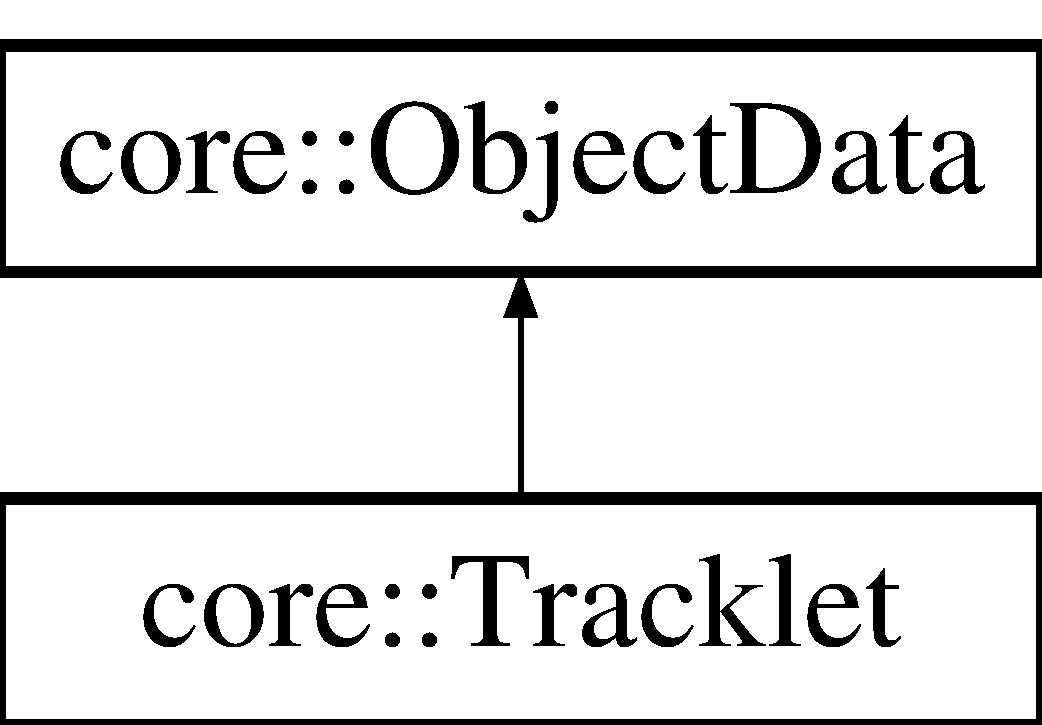
\includegraphics[height=2.000000cm]{classcore_1_1Tracklet}
\end{center}
\end{figure}
\subsection*{Public Member Functions}
\begin{DoxyCompactItemize}
\item 
\hyperlink{classcore_1_1Tracklet_aedf59b5a9a068a28bb7570f2a031d4e7}{Tracklet} ()
\item 
void \hyperlink{classcore_1_1Tracklet_ab0b397f2d0685a927de886dbd36c3bc8}{Add\+Path\+Object} (Object\+Data\+Ptr obj, bool overwrite=false)
\item 
size\+\_\+t \hyperlink{classcore_1_1Tracklet_a1b963319d6c65614baec02a925f31691}{Get\+First\+Frame\+Index} () const
\item 
size\+\_\+t \hyperlink{classcore_1_1Tracklet_ad8e195b523cf2021394455cc21867d96}{Get\+Last\+Frame\+Index} () const
\item 
Object\+Data\+Ptr \hyperlink{classcore_1_1Tracklet_a9758349e8f25c479ffc4b21a90149a81}{Get\+Path\+Object} (size\+\_\+t i)
\item 
size\+\_\+t \hyperlink{classcore_1_1Tracklet_aee4298a7b734b2b7533d4536006a8aa8}{Get\+Path\+Object\+Count} () const
\item 
void \hyperlink{classcore_1_1Tracklet_a10b56b608b24ef547550540e5a755bce}{Interpolate\+Missing\+Frames} ()
\item 
virtual double \hyperlink{classcore_1_1Tracklet_a0357f2fa173941800571432dcbc96dc2}{Compare\+To} (Object\+Data\+Ptr obj) const override
\item 
virtual Object\+Data\+Ptr \hyperlink{classcore_1_1Tracklet_a5fb5e6ab9df668c3477e8b52f115b188}{Interpolate} (Object\+Data\+Ptr obj, double fraction) const override
\item 
virtual void \hyperlink{classcore_1_1Tracklet_a85f92a4059bf89f24a83f28935675181}{Visualize} (cv\+::\+Mat \&image, cv\+::\+Scalar \&color) const override
\item 
void \hyperlink{classcore_1_1Tracklet_a3a2b241939559e47aef701d2e2c4d4bd}{Visualize} (cv\+::\+Mat \&image, cv\+::\+Scalar \&color, size\+\_\+t frame, size\+\_\+t predecessor\+\_\+count, size\+\_\+t successor\+\_\+count) const
\item 
void \hyperlink{classcore_1_1Tracklet_a2bdb2f2c8249145808e7029dde6e7df0}{Flatten} ()
\item 
void \hyperlink{classcore_1_1Tracklet_a5bbbf1e2858edaad93c04cc663afeeff}{Combine} (Tracklet\+Ptr other)
\item 
Object\+Data\+Ptr \hyperlink{classcore_1_1Tracklet_a5a0e56045f8c1868b46db87700658260}{Get\+Frame\+Object} (size\+\_\+t frame\+\_\+index)
\end{DoxyCompactItemize}


\subsection{Detailed Description}
A class for storing multiple object data objects. The object data objects are handled as a path. All objects are stored sorted ascending by their frame index. 

\subsection{Constructor \& Destructor Documentation}
\index{core\+::\+Tracklet@{core\+::\+Tracklet}!Tracklet@{Tracklet}}
\index{Tracklet@{Tracklet}!core\+::\+Tracklet@{core\+::\+Tracklet}}
\subsubsection[{\texorpdfstring{Tracklet()}{Tracklet()}}]{\setlength{\rightskip}{0pt plus 5cm}core\+::\+Tracklet\+::\+Tracklet (
\begin{DoxyParamCaption}
{}
\end{DoxyParamCaption}
)}\hypertarget{classcore_1_1Tracklet_aedf59b5a9a068a28bb7570f2a031d4e7}{}\label{classcore_1_1Tracklet_aedf59b5a9a068a28bb7570f2a031d4e7}
Creates a empty tracklet to store path object in. This is N\+OT a virtual object. 

\subsection{Member Function Documentation}
\index{core\+::\+Tracklet@{core\+::\+Tracklet}!Add\+Path\+Object@{Add\+Path\+Object}}
\index{Add\+Path\+Object@{Add\+Path\+Object}!core\+::\+Tracklet@{core\+::\+Tracklet}}
\subsubsection[{\texorpdfstring{Add\+Path\+Object(\+Object\+Data\+Ptr obj, bool overwrite=false)}{AddPathObject(ObjectDataPtr obj, bool overwrite=false)}}]{\setlength{\rightskip}{0pt plus 5cm}void core\+::\+Tracklet\+::\+Add\+Path\+Object (
\begin{DoxyParamCaption}
\item[{Object\+Data\+Ptr}]{obj, }
\item[{bool}]{overwrite = {\ttfamily false}}
\end{DoxyParamCaption}
)}\hypertarget{classcore_1_1Tracklet_ab0b397f2d0685a927de886dbd36c3bc8}{}\label{classcore_1_1Tracklet_ab0b397f2d0685a927de886dbd36c3bc8}
Adds the path object sorted into the tracklet. 
\begin{DoxyParams}{Parameters}
{\em obj} & The path object to add \\
\hline
{\em overwrite} & If true and an object in the same frame as the given object already exists, the old one will be replaced by the new one \\
\hline
\end{DoxyParams}
\index{core\+::\+Tracklet@{core\+::\+Tracklet}!Combine@{Combine}}
\index{Combine@{Combine}!core\+::\+Tracklet@{core\+::\+Tracklet}}
\subsubsection[{\texorpdfstring{Combine(\+Tracklet\+Ptr other)}{Combine(TrackletPtr other)}}]{\setlength{\rightskip}{0pt plus 5cm}void core\+::\+Tracklet\+::\+Combine (
\begin{DoxyParamCaption}
\item[{Tracklet\+Ptr}]{other}
\end{DoxyParamCaption}
)}\hypertarget{classcore_1_1Tracklet_a5bbbf1e2858edaad93c04cc663afeeff}{}\label{classcore_1_1Tracklet_a5bbbf1e2858edaad93c04cc663afeeff}
Copies all detections from the specified tracklet to this tracklet


\begin{DoxyParams}{Parameters}
{\em other} & The tracklet to copy the detections from \\
\hline
\end{DoxyParams}
\index{core\+::\+Tracklet@{core\+::\+Tracklet}!Compare\+To@{Compare\+To}}
\index{Compare\+To@{Compare\+To}!core\+::\+Tracklet@{core\+::\+Tracklet}}
\subsubsection[{\texorpdfstring{Compare\+To(\+Object\+Data\+Ptr obj) const override}{CompareTo(ObjectDataPtr obj) const override}}]{\setlength{\rightskip}{0pt plus 5cm}double core\+::\+Tracklet\+::\+Compare\+To (
\begin{DoxyParamCaption}
\item[{Object\+Data\+Ptr}]{obj}
\end{DoxyParamCaption}
) const\hspace{0.3cm}{\ttfamily [override]}, {\ttfamily [virtual]}}\hypertarget{classcore_1_1Tracklet_a0357f2fa173941800571432dcbc96dc2}{}\label{classcore_1_1Tracklet_a0357f2fa173941800571432dcbc96dc2}
Compares this object with the given object. 
\begin{DoxyParams}{Parameters}
{\em obj} & A pointer to the object to compare this object to \\
\hline
\end{DoxyParams}
\begin{DoxyReturn}{Returns}
A double value indicating the comparison result 
\end{DoxyReturn}


Reimplemented from \hyperlink{classcore_1_1ObjectData_afbf7a1e87235f1b204d4d2eb8a37a9a6}{core\+::\+Object\+Data}.

\index{core\+::\+Tracklet@{core\+::\+Tracklet}!Flatten@{Flatten}}
\index{Flatten@{Flatten}!core\+::\+Tracklet@{core\+::\+Tracklet}}
\subsubsection[{\texorpdfstring{Flatten()}{Flatten()}}]{\setlength{\rightskip}{0pt plus 5cm}void core\+::\+Tracklet\+::\+Flatten (
\begin{DoxyParamCaption}
{}
\end{DoxyParamCaption}
)}\hypertarget{classcore_1_1Tracklet_a2bdb2f2c8249145808e7029dde6e7df0}{}\label{classcore_1_1Tracklet_a2bdb2f2c8249145808e7029dde6e7df0}
Flattens the current tracklet one level. That means, that if this tracklet contains other tracklets as path objects, their path objects are all extracted and used as the new path objects of this tracklet. The old tracklet path objects are removed. \index{core\+::\+Tracklet@{core\+::\+Tracklet}!Get\+First\+Frame\+Index@{Get\+First\+Frame\+Index}}
\index{Get\+First\+Frame\+Index@{Get\+First\+Frame\+Index}!core\+::\+Tracklet@{core\+::\+Tracklet}}
\subsubsection[{\texorpdfstring{Get\+First\+Frame\+Index() const}{GetFirstFrameIndex() const}}]{\setlength{\rightskip}{0pt plus 5cm}size\+\_\+t core\+::\+Tracklet\+::\+Get\+First\+Frame\+Index (
\begin{DoxyParamCaption}
{}
\end{DoxyParamCaption}
) const}\hypertarget{classcore_1_1Tracklet_a1b963319d6c65614baec02a925f31691}{}\label{classcore_1_1Tracklet_a1b963319d6c65614baec02a925f31691}
Gets the lowest frame index of all path objects. \begin{DoxyReturn}{Returns}
The lowest frame index 
\end{DoxyReturn}
\index{core\+::\+Tracklet@{core\+::\+Tracklet}!Get\+Frame\+Object@{Get\+Frame\+Object}}
\index{Get\+Frame\+Object@{Get\+Frame\+Object}!core\+::\+Tracklet@{core\+::\+Tracklet}}
\subsubsection[{\texorpdfstring{Get\+Frame\+Object(size\+\_\+t frame\+\_\+index)}{GetFrameObject(size\_t frame\_index)}}]{\setlength{\rightskip}{0pt plus 5cm}Object\+Data\+Ptr core\+::\+Tracklet\+::\+Get\+Frame\+Object (
\begin{DoxyParamCaption}
\item[{size\+\_\+t}]{frame\+\_\+index}
\end{DoxyParamCaption}
)}\hypertarget{classcore_1_1Tracklet_a5a0e56045f8c1868b46db87700658260}{}\label{classcore_1_1Tracklet_a5a0e56045f8c1868b46db87700658260}
Gets the detected object at the given frame index or a nullptr if there is not detection.


\begin{DoxyParams}{Parameters}
{\em frame\+\_\+index} & The index of the frame to take the detection from \\
\hline
\end{DoxyParams}
\begin{DoxyReturn}{Returns}
A pointer to the detection in the given frame 
\end{DoxyReturn}
\index{core\+::\+Tracklet@{core\+::\+Tracklet}!Get\+Last\+Frame\+Index@{Get\+Last\+Frame\+Index}}
\index{Get\+Last\+Frame\+Index@{Get\+Last\+Frame\+Index}!core\+::\+Tracklet@{core\+::\+Tracklet}}
\subsubsection[{\texorpdfstring{Get\+Last\+Frame\+Index() const}{GetLastFrameIndex() const}}]{\setlength{\rightskip}{0pt plus 5cm}size\+\_\+t core\+::\+Tracklet\+::\+Get\+Last\+Frame\+Index (
\begin{DoxyParamCaption}
{}
\end{DoxyParamCaption}
) const}\hypertarget{classcore_1_1Tracklet_ad8e195b523cf2021394455cc21867d96}{}\label{classcore_1_1Tracklet_ad8e195b523cf2021394455cc21867d96}
Gets the highest frame index of all path objects. \begin{DoxyReturn}{Returns}
The highest frame index 
\end{DoxyReturn}
\index{core\+::\+Tracklet@{core\+::\+Tracklet}!Get\+Path\+Object@{Get\+Path\+Object}}
\index{Get\+Path\+Object@{Get\+Path\+Object}!core\+::\+Tracklet@{core\+::\+Tracklet}}
\subsubsection[{\texorpdfstring{Get\+Path\+Object(size\+\_\+t i)}{GetPathObject(size\_t i)}}]{\setlength{\rightskip}{0pt plus 5cm}Object\+Data\+Ptr core\+::\+Tracklet\+::\+Get\+Path\+Object (
\begin{DoxyParamCaption}
\item[{size\+\_\+t}]{i}
\end{DoxyParamCaption}
)}\hypertarget{classcore_1_1Tracklet_a9758349e8f25c479ffc4b21a90149a81}{}\label{classcore_1_1Tracklet_a9758349e8f25c479ffc4b21a90149a81}
Gets the path object at the given index. The index is N\+OT the frame index \begin{DoxyReturn}{Returns}
A pointer to the path object 
\end{DoxyReturn}
\index{core\+::\+Tracklet@{core\+::\+Tracklet}!Get\+Path\+Object\+Count@{Get\+Path\+Object\+Count}}
\index{Get\+Path\+Object\+Count@{Get\+Path\+Object\+Count}!core\+::\+Tracklet@{core\+::\+Tracklet}}
\subsubsection[{\texorpdfstring{Get\+Path\+Object\+Count() const}{GetPathObjectCount() const}}]{\setlength{\rightskip}{0pt plus 5cm}size\+\_\+t core\+::\+Tracklet\+::\+Get\+Path\+Object\+Count (
\begin{DoxyParamCaption}
{}
\end{DoxyParamCaption}
) const}\hypertarget{classcore_1_1Tracklet_aee4298a7b734b2b7533d4536006a8aa8}{}\label{classcore_1_1Tracklet_aee4298a7b734b2b7533d4536006a8aa8}
Gets the count of all path objects. \begin{DoxyReturn}{Returns}
The path object count 
\end{DoxyReturn}
\index{core\+::\+Tracklet@{core\+::\+Tracklet}!Interpolate@{Interpolate}}
\index{Interpolate@{Interpolate}!core\+::\+Tracklet@{core\+::\+Tracklet}}
\subsubsection[{\texorpdfstring{Interpolate(\+Object\+Data\+Ptr obj, double fraction) const override}{Interpolate(ObjectDataPtr obj, double fraction) const override}}]{\setlength{\rightskip}{0pt plus 5cm}Object\+Data\+Ptr core\+::\+Tracklet\+::\+Interpolate (
\begin{DoxyParamCaption}
\item[{Object\+Data\+Ptr}]{obj, }
\item[{double}]{fraction}
\end{DoxyParamCaption}
) const\hspace{0.3cm}{\ttfamily [override]}, {\ttfamily [virtual]}}\hypertarget{classcore_1_1Tracklet_a5fb5e6ab9df668c3477e8b52f115b188}{}\label{classcore_1_1Tracklet_a5fb5e6ab9df668c3477e8b52f115b188}
Linearly interpolates between this and the given object. Creates a new object to fit between the two objects. 
\begin{DoxyParams}{Parameters}
{\em obj} & A pointer to the target object \\
\hline
{\em fraction} & Describes where the interpolation should be done. A fraction of zero is a clone of this object, a fraction of one is a clone of the target object. \\
\hline
\end{DoxyParams}
\begin{DoxyReturn}{Returns}
The interpolated object 
\end{DoxyReturn}


Reimplemented from \hyperlink{classcore_1_1ObjectData_ad681915317decab76c384a635fc8444e}{core\+::\+Object\+Data}.

\index{core\+::\+Tracklet@{core\+::\+Tracklet}!Interpolate\+Missing\+Frames@{Interpolate\+Missing\+Frames}}
\index{Interpolate\+Missing\+Frames@{Interpolate\+Missing\+Frames}!core\+::\+Tracklet@{core\+::\+Tracklet}}
\subsubsection[{\texorpdfstring{Interpolate\+Missing\+Frames()}{InterpolateMissingFrames()}}]{\setlength{\rightskip}{0pt plus 5cm}void core\+::\+Tracklet\+::\+Interpolate\+Missing\+Frames (
\begin{DoxyParamCaption}
{}
\end{DoxyParamCaption}
)}\hypertarget{classcore_1_1Tracklet_a10b56b608b24ef547550540e5a755bce}{}\label{classcore_1_1Tracklet_a10b56b608b24ef547550540e5a755bce}
Interpolates between the current path objects until every missing frame has an object. Only frames between the first frame index and the last frame index are interpolated. \index{core\+::\+Tracklet@{core\+::\+Tracklet}!Visualize@{Visualize}}
\index{Visualize@{Visualize}!core\+::\+Tracklet@{core\+::\+Tracklet}}
\subsubsection[{\texorpdfstring{Visualize(cv\+::\+Mat \&image, cv\+::\+Scalar \&color) const override}{Visualize(cv::Mat \&image, cv::Scalar \&color) const override}}]{\setlength{\rightskip}{0pt plus 5cm}void core\+::\+Tracklet\+::\+Visualize (
\begin{DoxyParamCaption}
\item[{cv\+::\+Mat \&}]{image, }
\item[{cv\+::\+Scalar \&}]{color}
\end{DoxyParamCaption}
) const\hspace{0.3cm}{\ttfamily [override]}, {\ttfamily [virtual]}}\hypertarget{classcore_1_1Tracklet_a85f92a4059bf89f24a83f28935675181}{}\label{classcore_1_1Tracklet_a85f92a4059bf89f24a83f28935675181}
Visualizes the object in the given image with the given color. This method does nothing, it needs to be overwritten to visualize something. 
\begin{DoxyParams}{Parameters}
{\em image} & The image to write into \\
\hline
{\em color} & The color to use \\
\hline
\end{DoxyParams}


Reimplemented from \hyperlink{classcore_1_1ObjectData_aae2c4fceddc529570dbe8909309f9961}{core\+::\+Object\+Data}.

\index{core\+::\+Tracklet@{core\+::\+Tracklet}!Visualize@{Visualize}}
\index{Visualize@{Visualize}!core\+::\+Tracklet@{core\+::\+Tracklet}}
\subsubsection[{\texorpdfstring{Visualize(cv\+::\+Mat \&image, cv\+::\+Scalar \&color, size\+\_\+t frame, size\+\_\+t predecessor\+\_\+count, size\+\_\+t successor\+\_\+count) const}{Visualize(cv::Mat \&image, cv::Scalar \&color, size\_t frame, size\_t predecessor\_count, size\_t successor\_count) const}}]{\setlength{\rightskip}{0pt plus 5cm}void core\+::\+Tracklet\+::\+Visualize (
\begin{DoxyParamCaption}
\item[{cv\+::\+Mat \&}]{image, }
\item[{cv\+::\+Scalar \&}]{color, }
\item[{size\+\_\+t}]{frame, }
\item[{size\+\_\+t}]{predecessor\+\_\+count, }
\item[{size\+\_\+t}]{successor\+\_\+count}
\end{DoxyParamCaption}
) const}\hypertarget{classcore_1_1Tracklet_a3a2b241939559e47aef701d2e2c4d4bd}{}\label{classcore_1_1Tracklet_a3a2b241939559e47aef701d2e2c4d4bd}
Visualizes the tracklet by visualizing the path object in the given frame and the number of path objects in the given range before and after the given frame. 
\begin{DoxyParams}{Parameters}
{\em image} & The image to write into \\
\hline
{\em color} & The color to use \\
\hline
{\em frame} & The frame index to visualize the path objects from \\
\hline
{\em predecessor\+\_\+count} & The number of path objects to visualize before the given frame \\
\hline
{\em successor\+\_\+count} & The number of path objects to visualize after the given frame \\
\hline
\end{DoxyParams}


The documentation for this class was generated from the following files\+:\begin{DoxyCompactItemize}
\item 
core/Tracklet.\+h\item 
core/Tracklet.\+cpp\end{DoxyCompactItemize}

\hypertarget{classalgo_1_1TwoStage}{}\section{algo\+:\+:Two\+Stage Class Reference}
\label{classalgo_1_1TwoStage}\index{algo\+::\+Two\+Stage@{algo\+::\+Two\+Stage}}


{\ttfamily \#include $<$Two\+Stage.\+h$>$}

\subsection*{Public Member Functions}
\begin{DoxyCompactItemize}
\item 
\hyperlink{classalgo_1_1TwoStage_ae302f9ea93d56155a9dbd0be060500f7}{Two\+Stage} (size\+\_\+t max\+\_\+frame\+\_\+skip, double penalty\+\_\+value, size\+\_\+t max\+\_\+tracklet\+\_\+count)
\item 
void \hyperlink{classalgo_1_1TwoStage_a02dfe4e3fb244ecad13f676ce53d689a}{Create\+Object\+Graph} (Directed\+Graph \&graph, const \hyperlink{classcore_1_1DetectionSequence}{core\+::\+Detection\+Sequence} \&detections)
\item 
void \hyperlink{classalgo_1_1TwoStage_ae14cf79859b4275c862d6750b6bc6837}{Create\+Tracklet\+Graph} (Directed\+Graph \&obj\+\_\+graph, Directed\+Graph \&tlt\+\_\+graph, size\+\_\+t frame\+\_\+count)
\item 
void \hyperlink{classalgo_1_1TwoStage_a09168d0ace15d689c9d594ca16b93c38}{Extract\+Tracks} (Directed\+Graph \&tlt\+\_\+graph, size\+\_\+t depth, std\+::vector$<$ core\+::\+Tracklet\+Ptr $>$ \&tracks)
\end{DoxyCompactItemize}


\subsection{Detailed Description}
Implementation of the two-\/staged graph-\/based multi-\/object tracker. 

\subsection{Constructor \& Destructor Documentation}
\index{algo\+::\+Two\+Stage@{algo\+::\+Two\+Stage}!Two\+Stage@{Two\+Stage}}
\index{Two\+Stage@{Two\+Stage}!algo\+::\+Two\+Stage@{algo\+::\+Two\+Stage}}
\subsubsection[{\texorpdfstring{Two\+Stage(size\+\_\+t max\+\_\+frame\+\_\+skip, double penalty\+\_\+value, size\+\_\+t max\+\_\+tracklet\+\_\+count)}{TwoStage(size\_t max\_frame\_skip, double penalty\_value, size\_t max\_tracklet\_count)}}]{\setlength{\rightskip}{0pt plus 5cm}algo\+::\+Two\+Stage\+::\+Two\+Stage (
\begin{DoxyParamCaption}
\item[{size\+\_\+t}]{max\+\_\+frame\+\_\+skip, }
\item[{double}]{penalty\+\_\+value, }
\item[{size\+\_\+t}]{max\+\_\+tracklet\+\_\+count}
\end{DoxyParamCaption}
)}\hypertarget{classalgo_1_1TwoStage_ae302f9ea93d56155a9dbd0be060500f7}{}\label{classalgo_1_1TwoStage_ae302f9ea93d56155a9dbd0be060500f7}
Initializes the algorithm wih the given values. 
\begin{DoxyParams}{Parameters}
{\em max\+\_\+frame\+\_\+skip} & The maximum edge length to link objects \\
\hline
{\em penalty\+\_\+value} & The Edge value to link to source and sink \\
\hline
{\em max\+\_\+tracklet\+\_\+count} & The maximum number of tracklets to create \\
\hline
\end{DoxyParams}


\subsection{Member Function Documentation}
\index{algo\+::\+Two\+Stage@{algo\+::\+Two\+Stage}!Create\+Object\+Graph@{Create\+Object\+Graph}}
\index{Create\+Object\+Graph@{Create\+Object\+Graph}!algo\+::\+Two\+Stage@{algo\+::\+Two\+Stage}}
\subsubsection[{\texorpdfstring{Create\+Object\+Graph(\+Directed\+Graph \&graph, const core\+::\+Detection\+Sequence \&detections)}{CreateObjectGraph(DirectedGraph \&graph, const core::DetectionSequence \&detections)}}]{\setlength{\rightskip}{0pt plus 5cm}void algo\+::\+Two\+Stage\+::\+Create\+Object\+Graph (
\begin{DoxyParamCaption}
\item[{Directed\+Graph \&}]{graph, }
\item[{const {\bf core\+::\+Detection\+Sequence} \&}]{detections}
\end{DoxyParamCaption}
)}\hypertarget{classalgo_1_1TwoStage_a02dfe4e3fb244ecad13f676ce53d689a}{}\label{classalgo_1_1TwoStage_a02dfe4e3fb244ecad13f676ce53d689a}
Creates a graph with vertices for every detected object 
\begin{DoxyParams}{Parameters}
{\em graph} & The graph to write into \\
\hline
{\em detections} & The objects to use for the graph \\
\hline
\end{DoxyParams}
\index{algo\+::\+Two\+Stage@{algo\+::\+Two\+Stage}!Create\+Tracklet\+Graph@{Create\+Tracklet\+Graph}}
\index{Create\+Tracklet\+Graph@{Create\+Tracklet\+Graph}!algo\+::\+Two\+Stage@{algo\+::\+Two\+Stage}}
\subsubsection[{\texorpdfstring{Create\+Tracklet\+Graph(\+Directed\+Graph \&obj\+\_\+graph, Directed\+Graph \&tlt\+\_\+graph, size\+\_\+t frame\+\_\+count)}{CreateTrackletGraph(DirectedGraph \&obj\_graph, DirectedGraph \&tlt\_graph, size\_t frame\_count)}}]{\setlength{\rightskip}{0pt plus 5cm}void algo\+::\+Two\+Stage\+::\+Create\+Tracklet\+Graph (
\begin{DoxyParamCaption}
\item[{Directed\+Graph \&}]{obj\+\_\+graph, }
\item[{Directed\+Graph \&}]{tlt\+\_\+graph, }
\item[{size\+\_\+t}]{frame\+\_\+count}
\end{DoxyParamCaption}
)}\hypertarget{classalgo_1_1TwoStage_ae14cf79859b4275c862d6750b6bc6837}{}\label{classalgo_1_1TwoStage_ae14cf79859b4275c862d6750b6bc6837}
Reduces the object graph into linked tracklets. 
\begin{DoxyParams}{Parameters}
{\em obj\+\_\+graph} & The object graph to reduce \\
\hline
{\em tlt\+\_\+graph} & The graph to write the tracklets in \\
\hline
{\em frame\+\_\+count} & The frame count of the object graph \\
\hline
\end{DoxyParams}
\index{algo\+::\+Two\+Stage@{algo\+::\+Two\+Stage}!Extract\+Tracks@{Extract\+Tracks}}
\index{Extract\+Tracks@{Extract\+Tracks}!algo\+::\+Two\+Stage@{algo\+::\+Two\+Stage}}
\subsubsection[{\texorpdfstring{Extract\+Tracks(\+Directed\+Graph \&tlt\+\_\+graph, size\+\_\+t depth, std\+::vector$<$ core\+::\+Tracklet\+Ptr $>$ \&tracks)}{ExtractTracks(DirectedGraph \&tlt\_graph, size\_t depth, std::vector< core::TrackletPtr > \&tracks)}}]{\setlength{\rightskip}{0pt plus 5cm}void algo\+::\+Two\+Stage\+::\+Extract\+Tracks (
\begin{DoxyParamCaption}
\item[{Directed\+Graph \&}]{tlt\+\_\+graph, }
\item[{size\+\_\+t}]{depth, }
\item[{std\+::vector$<$ core\+::\+Tracklet\+Ptr $>$ \&}]{tracks}
\end{DoxyParamCaption}
)}\hypertarget{classalgo_1_1TwoStage_a09168d0ace15d689c9d594ca16b93c38}{}\label{classalgo_1_1TwoStage_a09168d0ace15d689c9d594ca16b93c38}
Extracts the finished tracks from the given tracklet graph. 
\begin{DoxyParams}{Parameters}
{\em tlt\+\_\+graph} & The tracklet graph to extract from \\
\hline
{\em depth} & The depth to flatten the tracklets to \\
\hline
{\em tracks} & The vector to write the extracted tracks in \\
\hline
\end{DoxyParams}


The documentation for this class was generated from the following files\+:\begin{DoxyCompactItemize}
\item 
algo/Two\+Stage.\+h\item 
algo/Two\+Stage.\+cpp\end{DoxyCompactItemize}

%--- End generated contents ---

% Index
\backmatter
\newpage
\phantomsection
\clearemptydoublepage
\addcontentsline{toc}{chapter}{Index}
\printindex

\end{document}
